%&pdflatex
\documentclass[a4paper,11pt,titlepage]{article}
%\usepackage[margin=2.5cm]{geometry}
\usepackage[T1]{fontenc}
\usepackage[english]{babel}
% usare latin1 con windows
\usepackage[utf8]{inputenc}
% usare utf8 con linux
%\usepackage[uft8]{inputenc}
\usepackage{color, graphicx}%per scrivere con diversi colori
\usepackage{hyperref}
\usepackage{faktor}
\usepackage[makeroom]{cancel}
\usepackage{pgfplots}
\usepgfplotslibrary{patchplots}
\usetikzlibrary{patterns, positioning, arrows}
\pgfplotsset{compat=1.15}
\usepackage{float, subcaption, braket, bbold, amssymb,amsthm,amsmath,mathtools, tikz-cd}



%%% Definizione degli ambienti tipo "Teorema"
%\newtheorem{theorem}{Theorem}[chapter]

%\theoremstyle{theorem}
%\newtheorem{lemma}[theorem]{Lemma}
%\newtheorem{proposition}[theorem]{Proposition}
%\newtheorem{corollary}[theorem]{Corollary}
%\theoremstyle{definition}
%\newtheorem{definition}[theorem]{Definition}
%\theoremstyle{remark}
%\newtheorem{remark}[theorem]{Remark}
%\newtheorem{example}[theorem]{Example}

\numberwithin{equation}{section}

\newtheorem{theorem}{Theorem}[section]
\newtheorem{corollary}[theorem]{Corollary}
\newtheorem{proposition}[theorem]{Proposition}
\newtheorem{lemma}[theorem]{Lemma}

\theoremstyle{definition}
\newtheorem{definition}[theorem]{Definition}

\theoremstyle{remark}
\newtheorem{remark}[theorem]{Remark}
\newtheorem{example}[theorem]{Example}



% aumenta la spaziatura
\linespread{1.2}

\DeclareMathOperator{\tr}{tr}
\DeclareMathOperator{\pr}{pr}
\DeclareMathOperator{\Der}{Der}
\DeclareMathOperator{\Diff}{Diff}
\DeclareMathOperator{\sgn}{sgn}
\DeclareMathOperator{\i2}{i}
\DeclareMathOperator{\d2}{d}
\newcommand{\rfield}{\mathbb{R}}


%\newcommand{\restrict}[2]{\left.{#1}\right|_{#2}}
\newcommand{\restrict}[2]{{#1}\raisebox{-.5ex}{$|$}_{#2}}

\begin{document}


\begin{titlepage}
\begin{center}
 {\huge\bfseries Notes \\ Differentiable Manifolds \\ LMU Munich WS 19 \\}
 % ----------------------------------------------------------------
 \vspace{1.5cm}
 %{\Large\bfseries }\\[5pt]
 flaviorossetti@outlook.com\\[14pt]
  \vfill
  Last version: \today
\end{center}
\end{titlepage}

\pagenumbering{Roman}
\newpage
\begin{center}
 {\huge\bfseries Don't trust these notes! \\}

  \vfill
\end{center}
\newpage

\newpage
\begin{center}
 { \textit{Many thanks to Raul Morral for his help to improve the script} \\}

  \vfill
\end{center}
\newpage

% indice

\tableofcontents
\clearpage

%%%%%%%%%%%%%%%%%%%%%%%%%%%%%%%%%%%%%%%%%%%%%%%%%%%%%%%%%%%%%%%%
\pagenumbering{arabic}

%\chapter{Part I}
\section{Intro}

From the Lee book \cite{Lee}: "The central idea of calculus is \textit{linear approximation}". A function of one variable can be approximated by its tangent line, a curve by a tangent vector (i.e. velocity vector), a surface in $\rfield^3$ can be approximated by its tangent plane, and a map from $\rfield^n$ to $\rfield^m$ by its total derivative.
Here it comes the importance of tangent spaces.

Main idea: in order to study tangent vectors, we identify them with "directional derivatives". In particular, there is a natural one-to-one correspondence between geometric tangent vectors and linear maps from $C^{\infty}(\rfield^n)$ to $\rfield$ satisfying the product rule. Such maps are called \textit{derivations}.


\begin{remark} \label{pointorvec}
\textbf{Points or vectors?} We can think of elements of $\rfield^n$ either as points or vectors. As points, their only property is their location, given by the coordinates $(x_1, \ldots, x_n)$ on a chosen basis. As vectors, they are characterized by a direction and a magnitude, but their location is irrelevant (translational invariance). So given $v \in \rfield^n, v=v^ie_i$, it can be seen as an arrow with its initial point anywhere in $\rfield^n$. So, if we think about a vector tangent to the border of the sphere at a point $a$, we imagine the vector as living in a copy of $\rfield^n$ with its origin translated to a.

\end{remark}
\newpage

\section{Quick review: Basic Algebraic Structures}

\begin{definition} [Operation]
Let $G$ be a set. $\cdot$ is called a (binary) operation on $G$ if it is a map
\begin{align*}
\cdot \, \colon G &\times G \longrightarrow G \\
(&a, b) \longmapsto a \cdot b
\end{align*}
Such a map is usually denoted by the symbol $\cdot$ or, analogously, with the symbol $+$.
\end{definition}

\begin{definition} [Group] Given a set $G$ and an operation $\cdot$ on such set, we will call such set with the operation  (i.e. the couple $(G, \cdot)$) a group if the following properties are satisfied (for $a, b, c \in G$):
\begin{itemize}
\item $ a \cdot b \in G$ (closure property, which often follows from the definition of our operation)
\item $a \cdot (b \cdot c) = (a \cdot b) \cdot c$ (associativity)
\item $\exists\, \mathbf{1} \in G$ such that $\mathbf{1} \cdot g = g, \, \forall\, g \in G$ (existence of the identity element)
\item $\forall\, g \in G, \exists\, g^{-1} \in G$ such that $g \cdot g^{-1} = g^{-1} \cdot g = \mathbf{1}$ (existence of the inverse element)
\end{itemize}
For the sake of simplicity, we will often call $G$ a group, without referring to the operation on it.
\end{definition}

\begin{example}
$(\mathbb{Z}, +)$ is a group.
\end{example}

\begin{example}
$(\mathbb{R}, +)$ is a group. Also: $(\mathbb{R}, \cdot)$ is a group.
\end{example}

\begin{example}
$(\mathbb{N}, +)$ is not a group!
\end{example}

\begin{remark}
The identity element of a group is often denoted as $\mathbf{1}$ if the operation is denoted by the symbol $\cdot$, whereas it is denoted as $\mathbf{0}$ if the operation is denoted by the symbol $+$.
In a similar way, the inverse element is often denoted as $g^{-1}$ if the operation is denoted by the symbol $\cdot$, whereas it is denoted as $-g$ if the operation is denoted by the symbol $+$.

\end{remark}

\begin{definition} [Abelian group]
A group $(G, \cdot)$ is called abelian if its elements commute according to the operation $\cdot$, i.e. $a \cdot b = b \cdot a, \forall \,  a, b \in G$.
\end{definition}

Often we can consider sets with two operations, like $(\mathbb{R}, + , \cdot)$. If they satisfy some properties, they are called rings. If they satisfy even more properties, they are called fields. In particular:

\begin{definition} [Ring]
Given a set $R$ and two operations: $+$ (usually called "additive operation") and $\cdot$ (called "multiplicative operation") on it, we will call the set with the two operations, i.e. $(R, +, \cdot)$, a ring if the following properties are satisfied:
\begin{itemize}
\item $(R, +)$ is an abelian group
\item $\cdot$ is associative, i.e. $a \cdot (b \cdot c) = (a \cdot b) \cdot c, \, \forall\, a, b, c, \in R$
\item the multiplicative identity $\mathbf{1}$ exists, i.e. $\exists\, \mathbf{1} \in R$ such that $\mathbf{1} \cdot r = r, \, \forall\, r \in R$
\item $\cdot$ is distributive with respect to $+$, i.e. $a \cdot (b + c) = a \cdot b + a \cdot c$
\end{itemize}
\end{definition}

\begin{definition} [Commutative ring] $(R, +, \cdot)$ is a commutative ring if the multiplication operation $\cdot$ is commutative
\end{definition}

\begin{definition} [Unitary ring]
$(R, +, \cdot)$ is a unitary ring if it contains the multiplication inverse, i.e. the inverse element according to the operation $\cdot$.
\end{definition}

\begin{definition} [Field]
A unitary, commutative ring is called a field.
\end{definition}

\begin{example}
The set of $2 \times 2$ matrices made by real coefficients is a ring with the operation of sum between matrices and with the matrix multiplication. The ring is not commutative because the matrix multiplication is not a commutative operation. Nor it is unitary, since not all the matrices are invertible.
\end{example}

\begin{example}
The set of $2 \times 2$ matrices made by real coefficients is a ring with the operation of sum between matrices and with the matrix multiplication. The ring is not commutative because the matrix multiplication is not a commutative operation. Nor it is unitary, since not all the matrices are invertible.
\end{example}

\begin{example}
$(\mathbb{Z}, +, \cdot)$ is a commutative ring. It is not unitary since the inverse element for $\cdot$ is often in the rational numbers, i.e. $3^{-1}$ is the multiplicative inverse of $3$.
\end{example}

\begin{example}
$(\mathbb{R}, +, \cdot)$ is a field
\end{example}
\newpage

\section{Quick review: Morphisms}
\begin{definition}[Homomorphism]
A homomorphism $h$ between two sets endowed with operations (think about two groups, for instance) is a map which preserves the operations, i.e.:
\begin{equation*}
h \colon (G, +) \longrightarrow (H, \circ)
\end{equation*}
such that $h(a + b) = h(a) \circ h(b), \forall\, a, b, \in G$, where $(G, +)$ and $(H, \circ)$ are two groups. The definition for rings and fields is analogous. Sometimes these maps are just called morphisms (there is some difference between morphisms and homomorphisms but it usually matters only if you are dealing with more abstract algebraic structures).
\end{definition}

And now, some particular types of homomorphisms.

\begin{remark} [Monomorphism, epimorphisms and isomorphisms]
A monomorphism is an injective homomorphism. An epimorphism is a surjective homomorphism. An isomorphism is a bijective homomorphism (thus, it is both a monomorphism and an epimorphism).
\end{remark}

\begin{remark} [Endomorphism, automorphism]
An endomorphism is a homomorphism from one algebraic structure to itself. If such morphism is bijective, it is called automorphism.
\end{remark}

\begin{remark}
Don't get confused with hom\textbf{e}omorphisms! A homeomorphism is a continuous and bijective map between two topological space, such that its inverse is also continuous. In general it is not a homomorphism (without the \textbf{e}), because a topological space is not necessarily associated with an operation on it. (However if it has an operation, the continuity of the map implies that it is also a homomorphism).
\end{remark}
\newpage

\section{Quick review: Equivalence Classes, Quotient Spaces}
\begin{definition}[Binary relation]
  Given a set $E$, a (binary) relation $\sim$ on $E$ is a set of couples $(a, b) \in E \times E$. In other words, a binary relation is a subset of $E \times E$. Moreover, if $(a, b) \in \, \sim\,  \subset E \times E$, we use the following notation: $a \sim b$.
\end{definition}

\begin{definition}[Equivalence relation]
  Given a set $E$, an equivalence relation $\sim$ is a binary relation which satisfies the following properties:
  \begin{itemize}
    \item $a \sim a, \forall\, a \in E$ (reflexive property)
    \item $a \sim b \Rightarrow b \sim a, \forall\, a, b \in E$ (symmetric property)
    \item $a \sim b, b \sim c \Rightarrow a \sim c, \forall \, a, b, c \in E$ (transitive property)
  \end{itemize}
\end{definition}

\begin{example}
  The following are examples (or counter-examples) of equivalence relations:
  \begin{itemize}
  \item "\textit{Being equal to}" (i.e. "$\sim$" is "$=$") is an equivalence relation on $\rfield$: $x=x \, \forall\, x \in \rfield; x=y \Rightarrow y=x \, \forall\, x, y \in \rfield$, etc.
  \item "\textit{Has the same birthday as}" on the set of all people in the world is an equivalence relation.
  \item "\textit{Having mutual friends on Facebook}" on the set of Facebook users is not an equivalence relation (there is some problem with transitive property)
  \item "\textit{Being greater or equal to}" on $\rfield$ is not an equivalence relation (it is not symmetric, however it is antisymmetric and so it is called "partial order relation")
\end{itemize}
\end{example}

\begin{definition}[Equivalence class]
  Given a set $E$ and an equivalence relation $\sim$ on $E$, the equivalence class of $x \in E$ is the set $[x]$, where
  \begin{equation}
    [x] \equiv \left \{ y \in E \,|\, y \sim x \right \}
  \end{equation}
  The equivalence class $[x]$ always contains $x$ itself, by definition of equivalence relation.
\end{definition}

\begin{example} \label{modulo4ex}
  If we consider the equivalence relation "$x \sim y$ if $x-y = 4n$ for some $n \in \mathbb{N} \cup \{0\}$" on the set of $\mathbb{Z}$, the equivalence class of 1 is $[1] = \{\ldots, -7, -3, 1, 5, 9, \ldots\}$. We can also write "$x-y = 4n$ for some $n$" as $x \equiv_4 y$ (congruence modulo $4$)
\end{example}

\begin{definition}[Quotient space]
  Given a set $E$, an equivalence relation $\sim$ on $E$, the quotient space with respect to $\sim$ is denoted by $\faktor{E}{\sim}$ and it is the set of all equivalence classes:
  \begin{equation}
     \faktor{E}{\sim} \equiv \left \{ [x] \,|\, x \in E \right \}
  \end{equation}
\end{definition}

\begin{example} \label{quotientexample}
  Let's consider two examples:
  \begin{itemize}
    \item If we consider the example \ref{modulo4ex}, $\faktor{\mathbb{Z}}{\sim} = \{[0], [1], [2], [3]\}$. In this case, we also write $\faktor{\mathbb{Z}}{\sim} = \faktor{\mathbb{Z}}{4\mathbb{Z}}$
    \item If $V$ is a vector space and $U$ is a vector subspace of $V$, then we can consider the equivalence relation "$x \sim y$ if $x-y \in U$". We notice that $x \sim x$ for each $x \in V$ since $x-x = 0 \in U$, because $U$ is a vector space as well. Then, $\faktor{V}{\sim}$ is isomorphic to $V'$, where $V'$ is $V$ without its subspace $U$ (every element of $U$ is identified with 0 in the quotient space, because every element of $U$ is in the same equivalence class of 0).
    \item If we consider two groups instead of vector spaces, finding the quotient space requires a bit more effort.
  \end{itemize}
\end{example}
\newpage

\section{Derivations}
\begin{definition}[Derivation] \label{derivation}
If $a$ is a point of $\rfield^n$, a map $v \colon C^{\infty}(\rfield^n) \rightarrow \rfield$ is called a \textit{derivation at a} if it is linear over $\rfield$ and satisfies the following product rule:
$$\restrict{v(fg)}{a} = \restrict{f}{a} \restrict{v(g)}{a} + \restrict{g}{a} \restrict{v(f)}{a}$$
\end{definition}

\begin{remark}
Directional derivatives obviously satisfy the above definition, and in these cases such a rule is also called Leibnitz rule.
\end{remark}

%\begin{definition} $T_{a}\rfield^n$ is the set of all derivations of $C^{\infty}(\rfield^n)$ at $a$. (And it is a vector space)
%\end{definition}
\newpage
\section{Multilinear Forms}

\begin{definition}[1-forms]
Given a  vector space $V$ on a field $K$, a 1-form (or linear form) $\varphi \colon V \rightarrow K$ is a linear function from $V$ to $K$. $V^*$ (also denoted by $\Lambda V^*$) is the set of all linear forms on $V$.
\end{definition}

\begin{remark}
  The set of linear forms on $V$ has the structure of a vector space. Indeed, if $\mathbb{K}$ is the field of the vector space $V$, $\forall\, a, a_1, a_2 \in \mathbb{K}, \forall\, \varphi, \varphi_1, \varphi_2 \in V^*$:
  \begin{enumerate}
    \item $a(\varphi_1 + \varphi_2) = a \varphi_1 + a\varphi_2$ (because we define the map $a_1\varphi_1 + a_2\varphi_2$ as $a_1\varphi_1 + a_2\varphi_2 (x) \equiv a_1 \varphi_1(x) + a_2 \varphi_2(x), \forall\, x \in V$)
    \item $(a+b)\varphi(x) = (a\varphi + b \varphi)(x)$
    \item $\varphi=0$ if $\varphi(x) = 0 \forall\, x \in V$
    \item $-\varphi(x) = \varphi(-x)$
    \item $\mathbb{1}\varphi(x) = \varphi(x)$
    \item $ab\varphi(x) = ba \varphi(x)$
  \end{enumerate}
\end{remark}

\begin{definition}[Dual basis]
If $\{e_i\}_{i=1, \ldots, n}$ is a basis of $V$, then $\{ e^{*i} \}_{i=1}^n \subseteq V^*$ is called the \textit{dual basis} if $e^{*i}(e_j) = \delta^i_j$.
\end{definition}

\begin{remark}
We could prove that the dual basis is indeed a basis of the dual space, so $\dim(V) = \dim(\Lambda V^*)$. Check proposition \ref{basisprop1}.
\end{remark}

\begin{example}
  Let's consider three examples.
  \begin{enumerate}
    \item $p \in \rfield^3$, fixed. Let $V_p$ be the vector space $V_p \equiv \{ q-p \,|\, q \in \rfield^3 \}$. We will also denote it by $T_p\rfield^3$. We notice that $V_p = T_p\rfield^3 = \rfield^3$ (It is trivial to verify the inclusions "$\subseteq$" and "$\supseteq$"). Let $\left \{ (e_i)_p \right \}_{i=1,2,3}$ be a basis for $V_p$. If we consider the dual space $V_p^*$, we notice that $\left \{(dx^i)_p \right\}_{i=1,2,3}$ is a dual basis, where $(dx^i)_p (e_j) = \frac{\partial}{\partial x^j} x^i$. The index position is just a matter of notation, for now. Then, we can show that $V_p$ and $V_p^*$ are isomorphic, and the isomorphism is:
    \begin{align}
      g \colon V_p &\rightarrow V_p^* \\
      x &\mapsto g(x, \cdot) \nonumber
    \end{align}
    where $g$ is the euclidean metric in $\rfield^3$, i.e. $g(x, y) = d(x, y) = \\ = \sqrt{(x_1 - y_1)^2 + (x_2 - y_2)^2 + (x_3 - y_3)^2}$
    \item $V = \left \{ M \in M_2(\mathbb{C}) \, | \, M^{\dagger} = M, \tr(M) = 0 \right \}$ is a vector field on $\rfield$, where
    $$M= \left ( \begin{matrix}
    a &b \\
    c &d
  \end{matrix}\right ), M^{\dagger}= \left (\begin{matrix}
    \bar a &\bar b \\
    \bar c &\bar d
    \end{matrix} \right ), a, \ldots, d \in \mathbb{C}$$

  A basis for $V$ is $\{\sigma_i\}_{i=1,2,3}$, where
  $$\sigma_1 = \left ( \begin{matrix}
  0\, &1 \\
  1\, &0
\end{matrix}
  \right), \sigma_2 = \left ( \begin{matrix}
  0 &i \\
  -i &0
\end{matrix}
  \right), \sigma_3 = \left ( \begin{matrix}
  1 &0 \\
  0 &-1
\end{matrix}
  \right)$$
  and a dual basis is given by $e^{*i}(e_j) = \frac{1}{2} \tr(e_i, e_j)$ (using the matrix product).
  \item Quantum Mechanics: $$V = \{ f \colon \rfield^3 \rightarrow \rfield \, | \, ||f|| = \int_{\rfield^3} |f|^2 d^3x < \infty \} = L^2(\rfield^3)$$ is a vector space. If we consider the Laplacian operator $\Delta = \frac{\partial^2}{(\partial x^1)^2} + \frac{\partial^2}{(\partial x^2)^2} + \frac{\partial^2}{(\partial x^3)^2}$, then a basis is given by $\{e_n\} = \{\frac{f_n}{||f_n||}\}$, where $f_n$ eigenfunctions of $\Delta$: $\Delta f_n = \lambda_n fn$.
  A dual basis is given by $e^{*n} = \int_{\rfield^3} e_n$
  Notice that both $V$ and $V^*$ are infinite-dimensional spaces.
  Some notations:
  $$e_n = |f_n \rangle, e^{*n} = \langle f_n |, e^{*n}(e_m) = \braket{f_n | f_m}$$
  \end{enumerate}
\end{example}


\begin{remark}\label{vectorasder}
Every vector in $\rfield^n$ about a point $p \in \rfield^n$ (i.e. such that its origin is the point $p$) "can be seen" as a derivation (cf. def. \ref{derivation}), i.e. as a directional derivative of a function evaluated at the point $p$. For the sake of simplicity, we think $p=0$ (but the following results are true $\forall \, p \in \rfield^n$).
The sentence "can be seen" means that there is an isomorphism $\psi$ associating such vectors to such linear forms. Let's construct this isomorphism in the following steps:

\begin{enumerate}
\item Because of linearity, we just need to define the isomorphism for the basis vectors $\{ e_i \}_{i=1,\ldots,n}$ of $\rfield^n$.
\item Given the vector $e_j$ of the canonical basis, we associate it with the derivation $\partial_{x_j}$ in 0:
\begin{align}
\restrict{\partial_{x_j}}{p=0} \equiv \restrict{\frac{\partial}{\partial x_j}}{p=0} \colon C^{\infty}(\rfield^n) &\rightarrow \rfield \\
f &\mapsto \restrict{\frac{\partial}{\partial x_j}}{0} (f) \equiv \frac{\partial f}{\partial x_j} (0) \nonumber
\end{align}

In particular, if $\Der(\rfield^n) = \{ \text{derivations on }\rfield^n\}$ $ = \{ v\colon C^{\infty}\rightarrow \rfield, \\ \text{satisfying Leibnitz rule}\}$, then the map:
\begin{equation}
   \rfield^n \overset{\psi}{\longleftrightarrow}\Der(\rfield^n)
\end{equation}
such that $\psi(e_j) = \restrict{\partial_{x_j}}{p=0}, \forall \, e_j$ basis vector, and with $\restrict{\partial_{x_j}}{p=0}$ partial derivative with respect to the $j$-th component, defines a linear map. Indeed, it is linear because of linearity of derivations, and since we defined its behaviour on the basis vectors, it is also defined for every vector of $\rfield^n$. In general we have $\psi(v)=\restrict{\partial_{v}}{p=0}$, where $\restrict{\partial_v}{p=0}$ is the directional derivative with respect to $v$. Moreover, $\Der(\rfield^n)$ is a vector space and we used the double arrow above because $\psi$ is an isomorphism, i.e. a bijective map which preserves operations from one space to the other. Here every derivative is evaluated at $p=0$. We notice that the point $p$ itself is not important for the directional derivative (the \textit{direction} in which we differentiate is the same for every point of the space), but $p$ is meaningful when we \textit{evaluate} the derivative of the function at that point. Indeed, $\restrict{\partial_x (x^2)}{x=0} \not = \restrict{\partial_x (x^2)}{x=1}$, even if we are differentiating along the $x$-axis in both cases.
\end{enumerate}


What is more: given $V_0$, the set of all the vectors about $0$, we can consider its dual space $V_0^*$. %interpretation?
What is a possible dual basis?  We want to find linear forms $$e^{*i} \colon V_0 \rightarrow \rfield$$ such that $e^{*i}(e_j) = \delta_j^i$.
We have just seen that we can consider vectors as directional derivatives. So, given $e_j$ vector of the canonical basis, we will call it $\restrict{\frac{\partial}{\partial x^j}}{0}$ (because of the isomorphism, they are quite the same mathematical object).
Now, we want that
\begin{equation} \label{dualbasisdelta}
e^{*i}\left( \restrict{\frac{\partial}{\partial x^j}}{0} \right) = \delta_j^i
\end{equation}
First, let's consider the \textit{coordinate function}:
\begin{align} \label{coofunc}
x_j \colon \rfield^n \rightarrow & \rfield \\
v=(v_1, \ldots, v_n) \mapsto &v_j \nonumber
\end{align}
where $v_1, \ldots, v_j$ are the coordinates of the vector $v$ in the canonical basis. The linear form $x_j$ returns the $j$-th coordinate of a vector. So, given a vector $v \in \rfield^n$, every coordinate $v_j$ can be seen as $v_j = x_j(v)$.
Now, let's just define
\begin{equation} \label{dualdef}
e^{*i}\left( \restrict{\frac{\partial}{\partial x^j}}{0} \right) \equiv \restrict{\frac{\partial}{\partial x^j}}{0} x_i =\restrict{\frac{\partial}{\partial x^j} x_i}{0} = \delta_j^i
\end{equation}
Where $x_i$ is the coordinate function defined above (remember: $\partial_{x_j}$ is a derivation, so it must be applied to functions!). Now, it might seem that $e^{*i}$ does not take a vector as argument, but rather a function. Actually, this problem is solved by the isomorphism between vectors and directional derivatives proved above. If $\psi$ is the name of such isomorphism, we could slightly change the definition \eqref{dualdef} in order to solve this ambiguity:
\begin{equation}
e^{*i}(e_j) \equiv \psi(e_j) (x_i)
\end{equation}
where $x_i$ is the $i$-th coordinate function and
\begin{equation}
\psi(e_j) = \restrict{\frac{\partial}{\partial x^j}}{0} = \restrict{\partial_{x_j}}{0}
\end{equation}
The vectors of the dual basis will also be called
\begin{equation}
  dx^i \equiv e^{*i}
\end{equation}
This will be important later: we will define exterior forms of degree $k$ and we'll use both notations. The set of all these forms is $\Lambda^k V^*$, and its basis is given by products (in particular, exterior products) of $e^{*i_1}, \ldots, e^{*i_k}$ (i.e. $dx^{i_1}, \ldots, dx^{i_k}$).
\end{remark}

\begin{definition} [Set of vector fields] \label{setsfields}
We denote by $\mathfrak{X}(\rfield^n)$ the set of al possible vector fields in $\rfield^n$, i.e.
\begin{align}
\mathfrak{X}(\rfield^n) = \text{Der}\mathbb{F}(\rfield^n) \equiv\{ v \colon \mathbb{F}(\rfield^n) \rightarrow \mathbb{F}(\rfield^n) \text{ such that } \nonumber \\
 v \text{ is } \rfield\text{-linear and } v(fg) = v(f)g + fv(g)  \}
\end{align}
where $\mathbb{F} \equiv \{$ functions $f\colon \rfield^n \rightarrow \rfield \}$.
\end{definition}

\begin{remark} [Fields vs. Derivations] \label{fieldsvsder}
  If $v$ is a vector field in $\rfield^n$, then $v$ assigns a vector to another vector of $\rfield^n$. So $v \colon \rfield^n \rightarrow \rfield^n$. So, the set of all vector fields should be (we will use a different symbol to denote it):
  $$X(\rfield^n) = \left \{ v \colon \rfield^n \rightarrow \rfield^n \right \}$$
  However, the definition \ref{setsfields} is a bit different. Why?
  The fact is, we can consider a vector of $\rfield^n$ as a directional derivative, cf. remark \ref{vectorasder} (we are not considering any fixed point here, but the results do not change). Now a derivation, as defined in def. \ref{derivation}, is a map $v \colon C^{\infty}(\rfield^n) \rightarrow \rfield$, i.e. we can say that a derivation is a very smooth element of $\mathbb{F}(\rfield^n) = \{ \text{functions } f \colon \rfield^n \rightarrow \rfield\}$. So, $\mathfrak{X}(\rfield^n) \cong X(\rfield^n)$ because we can associate a derivation of $\mathfrak{X}(\rfield^n)$ to each vector of $X(\rfield^n)$, and vice versa. Then we also explained why in the definition of $\mathfrak{X}( \rfield^n)$ every element must be $\rfield$-linear and satisfy the Leibnitz rule: it follows from the definition of derivations.

  Now, a question arises: given $v$ vector field, should we write $v(p)$ (i.e. it takes vectors as argument) or should we write $v(f)$ (i.e. it takes smooth functions as arguments)? The answer is: it depends on the case, since they are two different "$v$"s. Which is, we will use vectors when we think of $v$ as a function who takes elements of $\rfield^n$, and we will use functions in the other case. And we can choose which case to use, since we can identify every vector field with a derivation, and every derivation with a vector field (for more info, see pag. 181 of \cite{Lee}). Now, let us analyze how $v(f)$ is made in the latter case.
  Given $v \in \mathfrak{X}(\rfield^n), f: \rfield^n \rightarrow \rfield$, we define the function $v(f)$ as
  \begin{align} \label{vfpdef}
    v(f) \colon \rfield^n &\rightarrow \rfield \nonumber \\
    p & \mapsto v(f)(p) \equiv v_p f
  \end{align}
  Now, in coordinates:
  \begin{equation} \label{vfieldincoord}
    v(f)(p) = v_p f = v^i(p)(e_i)_p f = v^i(p) \restrict{\frac{\partial}{\partial x^i}}{p} f = v^i(p) \frac{\partial f}{\partial x^i} (p)
  \end{equation}
  where we used summation convention, and the fact that every vector basis $e_i$ can be seen as $\restrict{\partial_{x_i}}{p}$. We defined it in the right way because, as expected, we found that $v_p(f)$ is the directional derivative of $f$ in the direction of $v$, evaluated at $p$. So, in brief:
  \begin{itemize}
    \item $v(f)(p)$ is a number
    \item $v(f)(\cdot)$ is a function from $\rfield^n$ to $\rfield$
    \item $v(\cdot)$ is a function from $\mathbb{F}(\rfield^n)$ to $\mathbb{F}(\rfield^n)$
  \end{itemize}
We also notice that the mathematical object $e_i$ is not much different from $\restrict{(e_i)}{p}$ in this case: there is no difference if we think about them as directions, but it makes a difference if we think about them as directional derivatives, because the latter notation gives info about the point in which the derivative is evaluated. So, we add the pedix "$p$" in order to make the isomorphism between vectors and directional derivatives more explicit. Check also the remark \ref{pointorvec}.
\end{remark}

\begin{figure}[h]
     \centering
     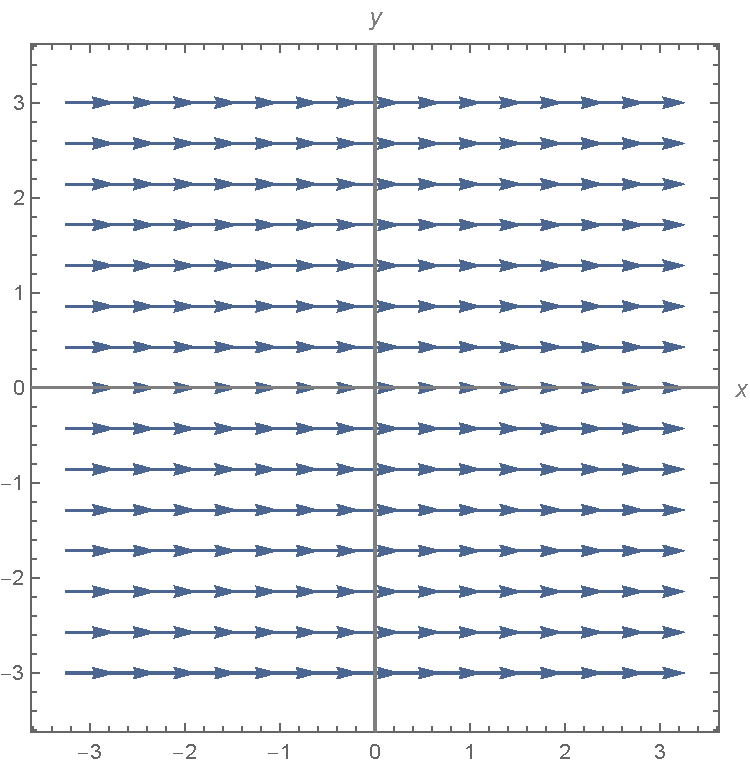
\includegraphics[width=.6\linewidth]{images/vfield_e1.pdf}
     \caption{Vector field v=$e_1=\partial_x$} \label{Fig:vfield_e1}
\end{figure}

%\begin{remark}
%So, if $v \in \mathfrak{X}(\rfield^n)$, then $v(f)(p) = \restrict{v(f)}{p} = v^i(p)\restrict{(e_i)}{p} = v^i(p) \restrict{\frac{\partial}{\partial x^i}}{p} f = v^i(p) \frac{\partial}{\partial x^i} f(p)$, where
%\end{remark}
\newpage
\section{Exterior Product and Generalisation}

\begin{definition} [Exterior form of degree $k$]
Given a vector space $V$ on a field $\mathbb{K}$, with $\dim(V) = n$, and with $k \le n$, an \textit{exterior form of degree $k$} (or $k$-linear form, or $k$-form) is a map $\omega$:
\begin{equation*}
\omega \colon \underbrace{V \times \ldots \times V}_{\text{k times}} \rightarrow \mathbb{K}
\end{equation*}
such that
\begin{equation*}
\omega(v_1, \ldots, v_k) = \sgn(\pi)\omega(v_{\pi(1)}, \ldots, v_{\pi(k)})
\end{equation*}
and such that $\omega$ is multilinear. Where $\pi$ is a permutation of $k$ elements, i.e. $\pi \in S_k$, and $\sgn(\pi)$ is the sign of the permutation.
We will also write $\omega \in \Lambda ^k V^*$.
\end{definition}

\begin{definition}[Exterior product between two 1-forms] \label{extprod}
Given a vector space $V$ on a field $\mathbb{K}, \dim(V) \ge 2$, and given $\varphi^1, \varphi^2 \in \Lambda V^* $, then we define the exterior product (or wedge product) $\wedge$ as:
\begin{align*}
\wedge \colon \Lambda V^* \times \Lambda V^* &\rightarrow \Lambda^2 V^*  \\
(\varphi^1, \varphi^2) &\mapsto \varphi^1 \wedge \varphi^2
\end{align*}
where:
\begin{equation*}
\varphi^1 \wedge \varphi^2 (x_1, x_2) = \varphi^1(x_1) \varphi^2(x_2) - \varphi^2(x_1) \varphi^1(x_2) = \det(\varphi^i (x_j))
\end{equation*}
for $i, j=1,2$.
\end{definition}

\begin{remark}[Exterior product between $k$ 1-forms]
The exterior product $\wedge$ that we defined for $k=2$ in \ref{extprod} is an exterior form of degree 2. We want to generalize it for $k$ vector spaces. In order to extend the definition, we want it to be an exterior form of degree $k$, so:
\begin{align*}
  \wedge \colon \underbrace{\Lambda V^* \times \ldots \times \Lambda V^*}_{k \text{ times}} &\rightarrow \Lambda^k V^*  \\
  (\varphi^1, \ldots, \varphi^k) &\mapsto \varphi^1 \wedge \ldots \wedge \varphi^k
\end{align*}
where, given $(x_1, \ldots, x_k) \in \underbrace{V \times \ldots \times V}_{k \text{ times}}$:
\begin{equation*}
  \varphi^1 \wedge \ldots \wedge \varphi^k (x_1, \ldots, x_k) =  \det(\varphi^i(x_j))
\end{equation*}
This is a particular case of an exterior $k$-form (because the sign of determinant changes if we swap two rows or two columns).
\end{remark}



\begin{proposition}\label{basisprop1}
  If $\{e_i\}_{i=1,\ldots,n}$ is a basis in $V$, then $\{e^{*i_1} \wedge \ldots \wedge e^{*i_k}\}_{i_1 < \ldots < i_k, k \le n}$ forms a basis of $\Lambda ^k V^*$
\end{proposition}

\begin{remark}
  The above proposition proves that $\dim(\Lambda^k V^*)=\binom{n}{k}$. Moreover, it means that any $\alpha \in \Lambda^k V^*$ can be written as:
  \begin{equation*}
    \alpha = \sum\limits_{i_1 < \ldots < i_k} a_{i_1 \cdots i_k} e^{*i_1} \wedge \cdots \wedge e^{*i_k}
  \end{equation*}
  where $a_{i_1 \cdots i_k} \in \mathbb{K}$, $\mathbb{K}$ field of the vector space.
\end{remark}

Now, we want to define the exterior product between a $k$-form and a $p$-form (and it will return a ($p+k$)-form).

\begin{definition}[Exterior product between a $k$-form and a $p$-form]
  Given $\alpha \in \Lambda ^k V^*, \beta \in \Lambda^p V^*$, the exterior product between them is defined as:
  \begin{align}
    \wedge \colon \Lambda ^k V^* \times \Lambda ^p V^* &\rightarrow \Lambda^{k+p} V^* \nonumber \\
    (\alpha, \beta) &\mapsto \alpha \wedge \beta \nonumber
  \end{align}
  with:
  $$\alpha \wedge \beta = \sum\limits_{\substack{i_1 < \ldots < i_k \\ j_1 < \ldots < j_p}} \alpha_{i_1 \cdots i_k}\beta_{j_1 \cdots j_k} e^{*i_1} \wedge \cdots \wedge e^{*i_k} \wedge e^{*j_1} \wedge \cdots \wedge e^{*j_k} $$
  where $\alpha_{i_1 \cdots i_k},\beta_{j_1 \cdots j_k} \in \mathbb{K}$
\end{definition}

\begin{example}[Oriented area]
  Let's consider the following examples:
  \begin{enumerate}
    \item $V = \rfield^3 \times \rfield^3$ with cartesian coordinates.
    $$\varphi \equiv dx^1 \wedge dx^2 + dx^2 \wedge dx^4$$
    Let's compute: $\varphi(e_i, e_j) = dx^1(e_i) dx^2(e_j) + dx^2(e_i)dx^4(e_j) + \\ - dx^2(e_i)dx^1(e_j) - dx^4(e_i)dx^2(e_j)$
    \item $V = \rfield^2$ with cartesian coordinates $x^1, x^2$.
    $$\varphi \equiv dx^1 \wedge dx^2$$
    Let's compute $\varphi(ae_1, be_2)$, where $ a,b \in \rfield$:
    \begin{align*}
    \varphi(ae_1, be_2) &= dx^1 \wedge dx^2(ae_1, be_2) = ab dx^1 \wedge dx^2(e_1, e_2) = \\
    &= ab (dx^1(e_1)dx^2(e_2) - \cancel{dx^2(e_1)} \cancel{dx^1(e^2)}) = ab = \\
    &= \text{oriented area of the rectangle of sides } a \text{ and } b
  \end{align*}
  \end{enumerate}

\end{example}

Let's check some properties about $k$-forms:
\begin{proposition}
  $\alpha \in \Lambda^k V^*, \beta \in \Lambda^p V^*, \gamma \in \Lambda ^q V^*$, then:
  \begin{enumerate}
    \item $(\alpha \wedge \beta) \wedge \gamma = \alpha \wedge (\beta \wedge \gamma)$
    \item $\alpha \wedge (\beta + \gamma) = \alpha \wedge \beta + \alpha \wedge \gamma$
    \item $\alpha \wedge \beta = (-1)^{kp} \beta \wedge \alpha$
  \end{enumerate}
\end{proposition}
\newpage
\section{Differential Forms}
\begin{definition} [Field of exterior forms, geometric definition] \label{geomkforms}
  (A field of) exterior forms of degree $k$, $k \le n$ is a map $\omega$ that associates to each point $p \in \rfield^n$ an element $\omega(p) \in \Lambda^{k}V_p^*$.
  Choosing a basis, we have:
  \begin{equation}
    \omega(p) = \sum\limits_{i_1 < \ldots < i_k} \underbrace{a_{i_1 \cdots i_k}(p)}_{\text{now it is a function!}} e^{*i_1} \wedge \cdots \wedge e^{*i_k}
    \end{equation}
    $\omega$ is a differential form if $a_{i_1 \cdots i_k}$ are differentiable. The set of differential $k$-forms is denoted by $\Omega^k(\rfield^n)$
\end{definition}

Another (equivalent) definition:

\begin{definition} [Algebraic definition of differential $k$-form] \label{algkforms}
  A differential $k$-form is a map:
  \begin{align}
    \underbrace{\mathfrak{X}(\rfield^n) \times \ldots \times \mathfrak{X}(\rfield^n)}_{k \text{ times}} \rightarrow \mathbb{F}(\rfield^n)
  \end{align}
  $C^\infty(\rfield^n)$ linear and alternating.
\end{definition}

\begin{remark}
  To show the equivalence of the two definition of differential $k$-forms we just need to show that:
  \begin{equation}
    \omega(p)(v_1, \ldots, v_k) = \omega(v_1, \ldots, v_k)(p)
  \end{equation}
\end{remark}

We want to generalize the concept of differential of a function.
\begin{definition}[Differential] \label{differential}
  Let $f$ be a function $f \colon U \subseteq \rfield^n \rightarrow \rfield$, $f$ differentiable. Let $v \in \mathfrak{X}(\rfield^n) = \Der \mathbb{F}(\rfield^n)$. The exterior derivative of $f$ is its differential $d$, defined as a 1-form such that:
  \begin{equation}
    df(v) = v(f)
  \end{equation}
\end{definition}

\begin{remark}[differential expression in coordinates]
  We want to verify that the above definition of differential is equivalent to our usual definition for $C^1(\rfield^n)$ function, which is:
  \begin{equation}
    df = \sum\limits_{i=1}^n \frac{\partial f}{\partial x_i} dx^i = \frac{\partial f}{\partial x_i} dx^i
  \end{equation}
  In order to prove that, we first consider a pointwise definition. Given $p \in \rfield^n$:
  \begin{equation} \label{diffdefp}
    df_p(v) = v(f), \forall\,\, v \in T_p \rfield^n \cong \rfield^n
  \end{equation}
  ($T_p \rfield^n$ is the tangent space to $\rfield^n$ at $p$). Now, we can write $v(f)$ in coordinates (the gray part is the one we don't care about):
  \begin{equation} \label{diffcoordinates}
    df_p = \textcolor{lightgray}{v(f) = \text{ }} v_i(p) (\lambda^i)_p
  \end{equation}
  where $(\lambda^i)_p$ is a dual basis at $p$ (later, we will prove that $(\lambda^i)_p = (dx^i)_p$). Now, applying $df$ to a particular vector (i.e. directional derivative) at $p$:
  \begin{equation} \label{diffpart1}
    df_p \left (\restrict{\frac{\partial}{\partial x^i}} {p} \right) = v_i(p)
  \end{equation}
  where we used the property of the dual basis
  \begin{equation}
    (\lambda^i)_p \restrict{\frac{\partial}{\partial x^j}} {p} = \delta^i_j
  \end{equation}
   and then:
   \begin{equation}
   \textcolor{lightgray}{df_p \left (\restrict{\frac{\partial}{\partial x^i}} {p} \right) = \text{ }} v_i(p) (\lambda^i)_p \restrict{\frac{\partial}{\partial x^i}} {p} = v_i(p)
 \end{equation}
   On the other hand, by definition \eqref{diffdefp} we know that:
   \begin{equation} \label{diffpart2}
     df_p \left (\restrict{\frac{\partial}{\partial x^i}} {p} \right)  = \restrict{\frac{\partial}{\partial x^i}} {p} f = \frac{\partial f}{\partial x^i} (p)
   \end{equation}
   Hence, using \eqref{diffpart1} and \eqref{diffpart2} we get:
   \begin{equation}
     v_i (p) = \frac{\partial f}{\partial x^i} (p)
   \end{equation}
   Then, by the expression of differential in coordinates \eqref{diffcoordinates}:
   \begin{equation}
     df_p = \frac{\partial f}{\partial x^i} (p) (\lambda^i)_p
   \end{equation}
   Applying the definition to $f = x^j$ (coordinate function, as defined in \eqref{coofunc}), we get:
   \begin{equation}
     df_p = \frac{\partial f}{\partial x^i} (p) (\lambda^i)_p = \frac{\partial f}{\partial x^i} (p) (dx^i)_p
   \end{equation}
   And then:
   \begin{equation}
     df = \frac{\partial f}{\partial x^i} dx^i
   \end{equation}
   Indeed, if $f = x^j$ then, as before:
   \begin{equation}
     (dx^j)_p = \frac{\partial x^j}{\partial x^i} (p) \restrict{(\lambda^i)}{p} = \delta^i_j \restrict{(\lambda^i)}{p} = \restrict{(\lambda^j)}{p}
   \end{equation}
Pay attention: what we did here is a bit different from what we did for the definition $\ref{vfpdef}$ of a vector field applied to a function. In this case, $p$ is the point where we fixed our vector, whereas in the other case $p$ was the point where we wanted to evaluate the directional derivative of $f$.
\end{remark}

In the above definition, $f$ was a 0-form (i.e. a function). What is the generalization of the differential to $k$-forms?

\begin{definition}[Exterior derivative] \label{extder}
  If $k > 0$, then the exterior derivative (acting on $k$-forms) is a map
  \begin{align*}
    \d2 \colon \Omega^k(\rfield^n) & \rightarrow \Omega^{k+1}(\rfield^n) \\
    \omega &\mapsto \d2 (\omega) \equiv \d2 \omega
  \end{align*}
  where
  \begin{equation*}
    \d2 \omega = \sum\limits_{j_1 < \ldots < j_k} \left (\d2 a_{j_1, \ldots, j_k} \right) \wedge dx^{j_1} \wedge \ldots \wedge dx^{j_k}
  \end{equation*}
With $\d2 a_{j_1, \ldots, j_k}$ differential of the function $a_{j_1, \ldots, j_k}$.
\end{definition}

\begin{example}[Computation of $d\omega$]
  Let's consider the following examples:
  \begin{enumerate}
    \item Let $\omega$ be a 2-form on $\rfield^3$ (coordinates $x^1, x^2, x^3$):
    $$\omega = dx^1 \wedge dx^2 + x^2 dx^1 \wedge dx^3$$
    Then
    $$\d2 \omega = dx^2 \wedge dx^1 \wedge dx^3$$
    where we used that $\d2 (dx^1 \wedge dx^2) = 0$ because there is no 3-form on a 2-dimensional space (otherwise, we can use that $d^2=0$, but we still have to prove it!)
    \item In $\rfield^n$, let's consider:
    $$\omega = x^2 dx^1, \d2 \omega = dx^2 \wedge dx^1$$
    where we computed  $\d2 \omega$ by using $\d2 g(v) = v(g)$ for a function $g$ and a vector field $v$. In fact, if $u,v \in \mathfrak{\rfield^n}$, then by definition of exterior product we have:
    $$\d2 \omega (u, v) = dx^2(u)dx^1(v) - dx^2(v)dx^1(u)$$
    On the other hand, using $dx^2(u)=u(x^2), v(x^2) = dx^2(v)$ (where $x^2$ is a function, the coordinate function defined in \eqref{coofunc}) we also have:
    $$\d2 \omega (u, v) = u(x^2)dx^1(v) - v(x^2)dx^2(u)$$
  \end{enumerate}
\end{example}

Some properties:
\begin{proposition}[Properties of exterior derivatives]
  $\omega_1 \in \Omega^k(\rfield^n), \omega_2 \in \Omega^p(\rfield^n)$. Then:
  \begin{itemize}
    \item $d(\omega_1 +\omega_2) = d\omega_1 + d\omega_2$
    \item $d(\omega_1 \wedge \omega_2) = d\omega_1 \wedge \omega_2 + (-1)^k \omega_1 \wedge d\omega_2$
    \item $d(d\omega_1)  = 0 = d(d\omega_2)$
  \end{itemize}
\end{proposition}

\begin{remark} \label{abusenot1}
  In the above proposition, we claimed that $d(d\omega)  = 0$ if $\omega \in \Omega^k(\rfield^n)$. The notation here is not the most precise, since the inner "d" is acting on a $k$-form, whereas the outer "d" is acting on a ($k+1$)-form (so, even if they share the same name, they are different maps). However the behaviour of both "d"s is clear, so we will continue with this abuse of notation.
\end{remark}

\begin{remark}
  The exterior derivative increases the degree of a $k$-form by 1 (the $k$-form becomes a ($k+1$)-form). Can we get backwards, which is, can we decrease the degree of a $k$-form? Answer: yes.
\end{remark}

\begin{definition}[Interior derivative] \label{intder}
  $z \in \mathfrak{X}(\rfield^n)$ (i.e. $z$ is a vector field), then we define the \textit{interior derivative} $i_z$ (acting on differential $k$-forms) as:
  \begin{align}
    \i2_z \colon \Omega^k(\rfield^n) &\rightarrow \Omega^{k-1}(\rfield^n) \\
    \omega &\mapsto \i2_z(\omega) \equiv \i2_z \omega \nonumber
  \end{align}
  where
  $$\i2_z \omega (v_1, \ldots, v_{k-1}) = \omega(z, v_1, \ldots, v_{k-1}), \forall \, v_i \in \mathfrak{X}(\rfield^n)$$
  $\i2_z \omega$ is also called the \textit{contraction} of $\omega$.
\end{definition}

\begin{example}[Some computations]
  In $\rfield^2$, $e_x, e_y$ basis vectors (that can be seen as vector fields):
  $$i_{e_x}(dx \wedge dy) = dy$$
  $$i_{e_y}(dx \wedge dy) = - dx$$
\end{example}

\begin{remark}
  In the definition \ref{intder} above, we used the algebraic definition of differential $k$-forms, i.e. definition \ref{algkforms}
\end{remark}

Now some properties for interior derivatives.

\begin{proposition}
  $\omega \in \Omega^k(\rfield^n), \eta \in \Omega^p(\rfield^n), z \in \mathfrak{X}(\rfield^n)$, then:
  \begin{itemize}
    \item $\i2_z (\omega \wedge \eta) = (\i2_z \omega) \wedge \eta + (-1)^k \omega \wedge (\i2_z \eta)$
    \item $\i2_z^2 w = \i2_z(\i2_z \omega) = 0$
  \end{itemize}
\end{proposition}

\begin{remark}
  In the above proposition there is a little abuse of notation when we claimed $\i2_z(\i2_z \omega) = 0$, see also remark \ref{abusenot1}.
\end{remark}

Now, let's talk about \textit{pullbacks} and \textit{pushforwards} for functions and $k$-forms.

\begin{definition}[Pullback]
  Let $f \colon U \rightarrow V$ (with $U, V \subseteq \rfield^n$) be a differentiable map. Let us suppose that $\dim(U) = \dim(V) = n$ (just for the sake of simplicity, since it is not necessary). Then the \textit{pullback} of a $k$-form (from $V$) to $U$ is the map:
  \begin{align*} \label{pullbackdef}
    f^* \colon \Omega^k(V) & \rightarrow \Omega^k(U) \\
    \omega & \mapsto f^*w
  \end{align*}
  such that
  \begin{equation*}
    (f^* \omega)(p) (u_1, \ldots, u_k) = \omega (f(p)) (df(u_1), \ldots, df(u_k)), \forall\, \, p \in \rfield^n, \forall \,\, u_i \in \mathfrak{X}(U)
  \end{equation*}
\end{definition}

Now, we want to give another name to the differential of a function.
\begin{definition}[Pushforward]
  Given $f \colon U \rightarrow V$ as before, we will also call the differential of $f$ at $p \in \rfield^n$, i.e. $df_p = df(p)$, as the \textit{pushforward} of $f$ at $p$, and it will be denoted by the symbol $(f_*)_p$.

  \textcolor{gray}{In our mind, we'll think of $df_p = (f_*)_p$, at least until this concept is generalized}.
\end{definition}

In particular, using the pullback definition above, we can write the pushforward map as:
\begin{align*}
  df_p \equiv (f_*)_p \colon U \subset \rfield^n &\rightarrow V \subset \rfield^m \\
    v & \mapsto (f_*)_p (v)
\end{align*}
By definition of differential, $df_p(v) = v(f)$, where $v$ is a vector tangent to $\rfield^n$ at $p$. Since vector are like directional derivatives, $v(f)$ is the directional derivative of $f$ with respect to $v$ (not evaluated at any point, for now!). In particular, if we apply the definition to a point $h(q)$, where $h \in C^{\infty}(\rfield^n, \rfield^m)$ (\textbf{CHECK}) and $q \in \rfield^n$, we have:
$$(f_*)_p (v)(h)(q) = (f_*)_p (v)(h(q)) = v(h(f(q))) = v(h \circ f) (q) = v (f^* h) (q)$$
In the last passage, we used the pullback for a differentiable function, which is completely legal since we defined it for differentiable $k$-forms, and a differentiable function is just a 0-form.

\begin{remark}
Using the pushforward, we can define the pullback of a differential form using a different notation (i.e. using $f_*$ instead of $df$):
  \begin{equation}
    (f^* \omega)(p) (u_1, \ldots, u_k) = \omega (f(p)) (f_*(u_1), \ldots, f_*(u_k)), \forall\, \, p \in \rfield^n, \forall \,\, u_i \in \mathfrak{X}(U)
  \end{equation}
\end{remark}

Now, some properties of the pullback.

\begin{proposition} \label{pullbackprop}
  $g, f \in C^1(\rfield^n, \rfield)$, $\omega, \varphi \in \Omega^k(\rfield^n)$, $h\colon \rfield^n \rightarrow \rfield$. Then:
  \begin{enumerate}
    \item $f^*(\omega + \varphi) = f^*(\omega) + f^*(\varphi)$
    \item $f^*(h \omega) = f^*(h)f^*(\omega)$
    \item $(f \circ g)^* = g^*(f^*(\omega))$
    \item If $\varphi^1, \ldots, \varphi^k \in \Omega^1(\rfield^n)$, then $f^*(\varphi^1 \wedge \ldots \wedge \varphi^k) = f^*(\varphi^1) \wedge \ldots \wedge f^*(\varphi^k)$
    \item $df^*(\omega) = f^*(d\omega)$
  \end{enumerate}
  From property (4) also follows that $f^*(\omega \wedge \phi) = (f^*\omega) \wedge (f^* \phi)$
\end{proposition}


\begin{remark}
We can express the pullback of a differential form in the following way:
\begin{align*}
(f^* \omega)(p) &= \sum\limits_{1 \le i_1 < i_2 < \cdots < i_k \le n} (f^*a_{i_1, \ldots i_k} (p)) f^*dy^{i_1} \wedge f^* dy^{i_2} \wedge \cdots \wedge f^* dy^{i_k} = \\
& = \sum\limits_{1 \le i_1 < i_2 < \cdots < i_k \le n} a_{i_1, \ldots, i_k} (f(p)) df^{i_1} \wedge df^{i_2} \wedge \cdots \wedge df^{i_k}
\end{align*}
where $f^i = y^i(f)$. We used properties (2) and (4) of proposition \ref{pullbackprop}
\end{remark}

\begin{remark}
  From our definition of pullback, it is not necessary that $f_*$ is invertible.
\end{remark}

\newpage
\section{Integration of differential forms}

Let $\omega$ be a differential form of degree $n$ in $\rfield^n$. Then $\omega$ is necessarily of the form
\begin{equation}
  \omega = \underbrace{a(p)}_{\text{it's a function}} dx^1 \wedge \ldots \wedge dx^n
\end{equation}
Such a form can be integrated:
\begin{equation}
  \int_{f(D)} \omega = \int_D f^* \omega
\end{equation}
\newpage
\section{More on Vector Fields}
\begin{definition}[Tangent space]
  $U \subset \rfield^n, U$ is an open set. $p \in U$, then the set of all derivations of $C^\infty(U)$ (cf. def \ref{derivation}) is called tangent space to $U$ at $p$ and is denoted by $T_p U$. An element of $T_p U$ is called a tangent vector at $p$, and it is often denoted by $v_p$.
\end{definition}


\begin{definition}[Tangent bundle]
The tangent bundle over an open subset $U \subset \mathbb{R}^n$ is defined as
\begin{equation}
	TU \equiv \underset{p \in U}{\sqcup} T_p U
\end{equation}
where $T_p U$ is the tangent space of $U$ at $p$. Every element of the disjoint union is represented by an ordered pair $(v, p)$ where $p \in U, v \in T_p U$.
The tangent bundle comes equipped with the projection map
\begin{align}
  \pr \colon TU &\rightarrow U \\
  (p, v) &\mapsto p \nonumber
\end{align}
So, every element of the tangent bundle is a couple made of a tangent space to a point, and the point itself.
\end{definition}

\begin{remark}
  In the previous definition, the "$\sqcup$" symbol denotes a disjoint union. "Disjoint" here means that, if we consider the disjoint union of two elements $x$ and $y$ such that $x=y$, the union is the set $\{x, y\}$ and not $\{x\} = \{y\}$ as in normal unions. The mathematical operator doesn't know if two elements are equal. Since we are not mathematical operators, we can enumerate the elements like: $\{(1, x), (2, y)\} = \{(1, x), (2, x)\} = \{(1, y), (2, y)\}$ in order to distinguish them.
\end{remark}

\begin{definition}[Alternative definition of vector field]
  A smooth vector field $v$ on $U \subset \rfield^n, U$ open, is a smooth map
  \begin{equation}
    v \colon U \rightarrow TU
  \end{equation}
  such that $\pr(v_p) = p, \forall \, p \in U$ %add command for pr
\end{definition}
\newpage
\begin{remark} [Space of sections]
  The set of all vector fields $\mathfrak{X}(U) \equiv \{ C^\infty(U, TU) \, | \\ \, \pr(v_p) = p \}$ is also called the space of sections in $TU$.
\end{remark}

\begin{definition} [Cotangent bundle]
  By duality we define
  \begin{equation}
    T^*U \equiv \underset{p \in U}{\sqcup} T_p^* U
  \end{equation}
  as the cotangent bundle. Where $T^*_p$, the dual space of the tangent space, is called cotangent space. We also associate a projection $\pr \colon T^*U \rightarrow U$ with it.
\end{definition}

Now, let's talk about about Lie algebras.

\begin{definition}[Lie algebra]
  A Lie algebra $(V, [\cdot, \, \cdot])$ is a vector space $V$ over $\rfield$ endowed with a map
  $$[\cdot , \, \cdot] \colon V \times V \rightarrow V$$
  with the following properties:
  \begin{itemize}
    \item $[\cdot , \, \cdot]$ is bilinear
    \item $[\cdot , \, \cdot]$ is antisymmetric ($[u, v] = -[v, u], \forall \, u, v \in V$)
    \item $[\cdot , \, \cdot]$ satisfies the \textit{Jacobi identity}:
    $$[[u, v], z] + [[z, u], v] + [[v, z], u] = 0$$
  \end{itemize}
\end{definition}

\begin{remark}[Jacobi]
  How to remember Jacobi identity: remember $[[u, v], z]$ and then  permute cyclically.
\end{remark}

\begin{proposition}
  $\mathfrak{X}(\rfield^n)$ is an (infinite dimensional) Lie algebra with $[u, v](f) = u(v(f)) - v(u(f))$, for $u, v \in \mathfrak{X}(\rfield^n), f \in C^\infty(\rfield^n)$. (Note that $u$ and $v$ are vector fields and $[u, v]$ is still a vector field).
\end{proposition}

\begin{definition}[Integral curve]
  An integral curve for a vector field $v$ is a smooth curve $\phi \colon (a, b) \rightarrow \rfield^n$ satisfying $\dot\phi(t) = v_{\phi(t)}$ ($v_{\phi(t)}$ is the vector tangent at $\phi(t)$ for $t$ fixed, remember the previous notation!). Let us suppose $0 \in (a, b)$. Then, $\phi(0)$ is called the starting point of $\phi$.
\end{definition}

We can also visualize the family of integral curves in the following way.

\begin{definition}[Flow]
  The map
  \begin{align}
    \theta \colon \rfield \times \rfield^n &\rightarrow \rfield^n \\
    (t, p) &\mapsto \theta_t(p) \nonumber
  \end{align}
  such that $\dot\theta_t(p) = v_{\theta_t(p)}$ is the flow of the vector field $v$ where, if we fix $p$, $\theta_t(p)$ is the integral curve which passes through $p$ at $t=0 \in (a, b)$.
  So the flow satisfies two conditions:
  \begin{align}
    \dot\theta_t(p) &= v_{\theta_t(p)} , \, &\forall \, p \in \rfield^n \\
    \theta_0(p) &= p, \, &\forall \, p \in \rfield^n
  \end{align}
Under the right hypothesis (e.g. Lipschitz hypothesis and smoothness of $v$) we can prove existence and uniqueness of the solution of such ODEs ($\forall p \in \rfield^n$).

By fixing either the time or the starting point of the flow, we can consider two maps:
\begin{itemize}
\item $p \mapsto \theta_t(p)$, for each fixed $t$ (we are observing several integral curves at the same time $t$)
\item $t \mapsto \theta_t(p)$, for each fixed $p$ (we are observing the integral curve starting from $p$, for all times)
\end{itemize}
\begin{figure}[h]
     \centering
     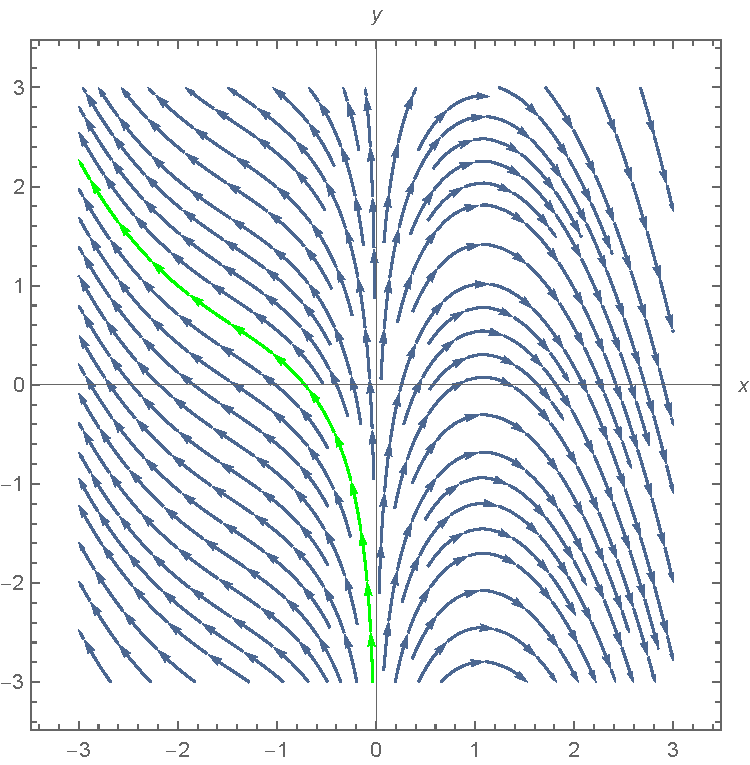
\includegraphics[width=.6\linewidth]{images/integralcurve_1.pdf}
     \caption{the map $t \mapsto \theta_t(p)$ selects just one integral curve} \label{Fig:integralcurve_1}
\end{figure}
\end{definition}

\begin{definition}[Lie derivative]
  Let $z \in \mathfrak{X}(\rfield^n)$ be a differentiable vector field, $\phi_t$ its flow and $\omega \in \Omega^k(\rfield^n)$. Then the Lie derivative of $\omega$ is defined as
  \begin{equation}
    L_z \omega = \restrict{\frac{d}{dt}(\phi_t^* \omega)}{t=0}
  \end{equation}
\end{definition}

\begin{remark}
  We denoted the flow by the symbol $\phi_t$ and not $\phi$. What we are doing here is not caring about $p$: $\phi^*_t \omega (\cdot) = \omega(\phi_t(\cdot))$
  %In components we have: ...to do
  Useful formula: $L_z \omega = (\d2 \i2_z + \i2_z \d2) \omega$
\end{remark}
\newpage
\section{Lie derivative of a vector field}
\begin{definition}[pullback of a vector field]
  %(move all definitions of pullback together)
  Let $\varphi$ be a diffeomorphism of $\rfield^n$ (i.e. a differentiable and invertible map from $\rfield^n$ to $\rfield^n$, such that its inverse is differentiable as well). Let $v \in \mathfrak{X}(\rfield^n)$. Then:
  \begin{equation}
    \varphi ^* v \equiv \varphi_* ^{-1}v
  \end{equation}
  is the pullback of $v$ with $\varphi$.
  In particular, given a flow $\phi$ and $t$ fixed, $\phi(t, \cdot) = \phi_t(\cdot)$ is a diffeomorphism on $\rfield^n$ with $\phi^{-1} = \phi(-t, \cdot) = \phi_{-t}(\cdot)$.
\end{definition}

\begin{definition}[Lie derivative of a vector field]
Let $u, v \in \mathfrak{X}(\rfield^n)$. The Lie derivative of $v$ in direction $u$ is
\begin{equation}
  L_u v \equiv \restrict{\frac{d}{dt}( \phi_t^* v)}{t=0}
\end{equation}
(Remember: $\phi\colon (t, p) \mapsto \phi(t, p), \phi_t^*v \colon (t, p) \mapsto v(\phi (t, p))$).
\end{definition}

\begin{lemma}
  Let $u, v$ be smooth vector fields on $\rfield^n$ and $\varphi \in \Diff(\rfield^n)$. Let $\phi_t$ be the flow of $u$ and let $\psi_s$ be the flow of $v$. Then
  \begin{itemize}
    \item $\varphi^*v = \restrict{\frac{d}{ds}}{s=0} \varphi^{-1} \circ \psi_s \circ \varphi$
    \item $\varphi^*v = v \Leftrightarrow \varphi \circ \psi_s = \psi_s \circ \varphi$ for all $s$.
    \item $L_u v = 0 \Leftrightarrow \phi_t \circ \psi_s = \psi_s \circ \phi_t$ for all $s, t$
  \end{itemize}
\end{lemma}

\begin{lemma}
  Let $u, v$ be smooth vector fields on $\rfield^n$ and and let $\phi_t$ (respectively $\psi_s$) be the flow of $u$ (respectively $v$). Then:
  \begin{itemize}
    \item $L_u v = \restrict{\frac{\partial^2}{\partial s \partial t} \phi_{-t} \circ \psi_s \circ \phi_t}{t=0,s=0}$
    \item $(L_u v) (f) = [u, v](f) = u(v(f)) - v(u(f))$ for all smooth functions $f$ on $\rfield^n$
  \end{itemize}
\end{lemma}

\begin{lemma}
  Let $u, v$ be smooth vector fields on $\rfield^n$ and $\varphi \in \Diff(\rfield^n)$. Then:
  \begin{enumerate}
    \item $[u, v]$ is $\rfield-$bilinear (i.e. bilinear for a parameter $\lambda \in \rfield$)
    \item $[u, v] = - [v, u]$
    \item The Jacobi identity holds
    \item $[u, fv] = f[u, v] + u(f)v$
    \item $\varphi_*[u, v] = [\varphi_* v, \varphi_* u]$
  \end{enumerate}
\end{lemma}
\newpage
  \section{Stokes' Theorem on $\rfield^n$}

\begin{itemize}
  \item For a function $f$ (i.e. a 0-form) on $[a, b] \subset \rfield$ we have $\int_a^b df = \int_a^b \partial_x f dx = f(b) - f(a)$ (fundamental theorem of calculus).
  \item for $\omega = a_i dx^i$, a 1-form on $U = [0, 1] \times [0, 1] \subset \rfield^2$ we have:
  $$\int_S d\omega = \int_S (\partial_{x^1} a_2) dx^1 \wedge dx^2 + (\partial_x^2 a_1) dx^2 \wedge dx^1 = \int_{\partial S} w$$
  where we used the fundamental theorem of calculus.
  \item More generally, if $S$ is a compact subset of $\rfield^2$ with piecewise regular boundary $\partial S$ (piecewise homeomorphic to intervals in $\rfield$) then we obtain by decomposing $S$ in terms of little squares and interpreting $\int_U d\omega$ as a Riemann sum over the square the result
  $$\int_U d\omega = \int_{\partial U} \omega$$
  This result generalizes immediately to compact co-dimension zero subsets of $\rfield^n$ with piecewise regulary boundary
  \item If $M$ is a compact subset of dimension $m \le n$ in $\rfield^n$ (with piecewise regular boundary $\partial M$), diffeomorphic to a compact subset of $U \subset \rfield^m$ (i.e. $M = f(U)$) and $\omega \in \Omega^{m-1}(M)$, then:
  $$\int_M d\omega = \int_U f^* d\omega = \int_U df^* \omega = \int_{\partial U} f^* \omega = \int_{\partial M} \omega$$
  \item More generally, the parametrization of $\partial M$ may be different from that induced by $M$. Then we have:
  $$\int_M d\omega = \int_{\partial M} i^* \omega$$
  where $i \colon \partial M \rightarrow M$ is the inclusion map of $\partial M$ into $M$.
\end{itemize}

So, the most general result that we achieved is the following:

\begin{theorem}[Stokes]
  $\omega \in \Omega^{m-1}(\rfield^n)$. Let $M$ be a closed compact subset of $\rfield^n$, $dim(M) = m \le n$, such that $M$ is homeomorphic to a closed subset $U \subset \rfield^m$. $\partial M$ is the boundary of $M$ and $i \colon \partial M \rightarrow M$ is the inclusion map of $\partial M$ into $M$. Then:
  \begin{equation}
    \int_{\partial M} i^* \omega = \int_M d\omega
  \end{equation}
\end{theorem}

\begin{corollary}[Fundamental theorem of line integrals]
  Let $f$ be a smooth function defined near an oriented curve $C$ in $\rfield^n$, with endpoints $A$ and $B$.
  Then:
  \begin{equation}
    \int df = \int \nabla f \cdot dx = f(B)-f(A) % TODO: add parametrization
  \end{equation}
\end{corollary}

\begin{corollary}[Curl theorem or Classical Stokes theorem]
  Let $v$ be a differentiable vector field defined near a surface $S \subset \rfield^3$ with boundary $\partial S$.
  \begin{equation}
    \int_S n \cdot (\nabla \times v)  dS = \int_{\partial S} v \cdot dx
  \end{equation}
  where $n$ is the normal vector on the surface at each point.
\end{corollary}

\begin{corollary}[Divergence theorem]
  For a smooth vector field $v$ defined on a solid $T \subset \rfield^3$ with boundary $\partial T$:
  \begin{equation}
    \int_T \nabla \cdot v \, dV = \int_{\partial T} v \cdot n \, dS
  \end{equation}
  where $dV$ is the unoriented volume element.
\end{corollary}
\newpage
\section{Poincarè Theorem of 1-forms}
\begin{definition} [Closed and exact forms]
  If $\omega \in \Omega^{k}(U)$ such that $\d2\omega = 0$, then $\omega$ is closed. If there exists $\alpha \in \Omega ^{k-1}(V), V \subset U$ such that $\omega = \d2\alpha$ in $V$ then $\omega$ is exact.
\end{definition}

\begin{proposition}
  The following are equivalent:
  \begin{enumerate}
    \item $\omega \in \Omega^1(U)$ is exact in a connected open subset $V \subset U$
    \item For any curve $\gamma \colon (a, b) \rightarrow U, \int_{\gamma} \omega$ depends only on the endpoints $\gamma(a)$ and $\gamma(b)$.
    \item $\int_{\gamma} \omega = 0$ for any closed curve $\gamma$ in $V$
  \end{enumerate}
\end{proposition}

\begin{remark}[A closed form is not always exact]
  If $\omega$ is exact, then it is closed (because $d^2=0$). But not every closed form in $\Omega^1(U), U$ open subset of $\rfield^n$ is exact. Cf. $\omega = - \frac{y}{x^2 + y^2} dx + \frac{x}{x^2+y^2}dy$ in $\rfield^2$ minus the non-negative $x$-axis. If $\gamma$ is a closed curve around the origin of $\rfield^2$, we have:
  $$\int_{\gamma} \omega = \int_{\gamma} d\theta = 2\pi$$
  and therefore $\omega$ cannot be exact by the previous proposition. However, we notice that we have problems only with the origin of $\rfield^2$. If we consider a subset of $\rfield^2$ which is enough far from the origin, the form would be an exact form in such subset. Indeed, we say that $\omega$ is locally exact, and the general result follows from the next theorem.
\end{remark}

\begin{theorem}[Poincarè theorem for 1-forms on $\rfield^n$]
  Let $\omega \in \Omega^1(U), U \subset \rfield^n, U$ open. Then $d\omega = 0$ if and only if for each $p \in U$ there is a neighbourhood $V \subset U$ of $p$ and a differentiable function $f \colon V \rightarrow \rfield$ such that $\omega = df$.
\end{theorem}

\begin{remark}
  Using the Poincarè theorem for 1-forms, we can extend the definition of the integral of a closed 1-form along a \textbf{continuous} path (until now, we have always assumed the our paths were piecewise differentiable). In fact, assume that $ \omega \in \Omega^1(U), \d2 \omega = 0$, and $\gamma$ such that:
  $$\gamma \colon [0, 1] \rightarrow U$$ is a differentiable map.
  Now, we choose a partition of $[0, 1]$, i.e. a collection of points $0 = t_0 < t_1 < \ldots < t_k < t_{k+1} = 1$ such that the restriction of $\gamma$ to the interval $(t_i, t_{i+1})$ is contained in a ball $B_i$ where $\omega$ is exact. In particular:
  $$\omega = df_i, \text{ for } f_i \colon B_i \rightarrow \rfield$$
  Then:
  $$\int_{\gamma} \omega = \sum_i \left[ f_i(t_{i+1}) - f_i(t_i) \right ]$$
  If $\gamma$ is only continuous, we could still consider such a partition, and still define
  $$\int_{\gamma} \omega = \sum_i \left[ f_i(t_{i+1}) - f_i(t_i) \right ]$$
  The integral of $\gamma$ is well defined because the definition is independent from the choice of our partition: if $P$ is one partition and $P'$ is a refinement of $P$ (i.e. it is the same partition plus an extra point $t' \in (t_i, t_{i+1})$ for some $i$), then:
  $$[f_i(t_{i+1}) - \cancel{f_i(t')}] + [\cancel{f_i(t')} - f_i(t_i)] = [f_i(t_{i+1}) - f_i(t_i)]$$
  Then the integral does not change if we consider a refinement. If we consider a general partition $P'$, we can add every point of the partition $P$ to $P'$, so that we get a refinement of $P'$ that we will be called $P''$. The integral on the partition $P'$ has the same value of the integral on the partition $P''$ by the above argument. Now, we can add every point of the partition $P'$ to $P$, so to get the partition $P''$ again, but now we can see $P''$ as a refinement of $P$. Then the integral on $P$ and on $P''$ are the same. Then also the integrals on $P$ and $P'$ are the same.
\end{remark}

Now, we want to extend the above theorem to $k$-forms.

\begin{definition} [Contractible set]
  An open subset $U \subset \rfield^n$ is contractible to some point $p_0 \in U$ if there exists a differentiable map
  \begin{align}
    H \colon U \times R &\rightarrow U \\
    (p,t) &\mapsto H(p, t) \nonumber
  \end{align}
  such that $H(p, 1) = p, H(p, 0) = p_0, \forall\, p \in U$
\end{definition}

\begin{remark}
  To every $\omega \in \Omega^k(U)$ we can associate a $k$-form $\bar\omega \in \Omega^k(U \times \rfield)$ defined as
  \begin{equation}
    \bar\omega = H^* \omega
  \end{equation}
  On the other hand, any $\bar \omega \in \Omega^k(U \times \rfield)$ has a unique decomposition of the form
  \begin{equation}
    \bar \omega = \omega_1 + dt \wedge \eta
  \end{equation}
  with $i_{\partial_t} \omega_1 = 0$ and $i_{\partial_t} \eta_1 = 0$.
  Conversely, we can associate a $k$-form $\omega \in \Omega^k(U)$ to each $\bar \omega \in \Omega^k(U \times \rfield)$ with the help of the inclusion map
  \begin{align}
    i_t \colon U &\rightarrow U \times \rfield \\
    p &\mapsto i_t(p) = (p,t)\nonumber
  \end{align}
  Then, $i_t^* \bar \omega \in \Omega^k(U)$ if $\bar \omega \in \Omega^k(U \times \rfield)$

  Furthermore, let's define the map
  \begin{align}
    I \colon \Omega^k(U \times \rfield) &\rightarrow \Omega^{k-1}(U) \\
    \eta &\mapsto I\eta \nonumber
  \end{align}
  such that $$(I\eta)(z_1, \ldots, z_{k-1}) = \int_0^1 \eta(p, t)(\partial_t, i_{t^*}z_1, \ldots, i_{t^*}z_{k-1})dt$$
\end{remark}

\begin{proof}
  Let's choose coordinates $\{x^1, \ldots, x^n, t\}$ for $U \times \rfield$. Then we write $\bar \omega$ on the basis:
  $$\bar \omega = \sum\limits_{i_1 < \ldots < i_k} a_{i_1 \cdots i_k} dx^{i_1} \wedge \ldots \wedge dx^{i_k} + \sum_{i_1 < \ldots < i_{k-1}} b_{i_1 \ldots i_{k-1}} dt \wedge dx^{i_1} \wedge \ldots \wedge dx^{i_{k-1}}$$
  (We can always do this, the coefficients could also be trivial).
  Now, we want to integrate this form. Let:
  \begin{align*}
    i_t \colon U &\rightarrow U \times \rfield \\
    p &\mapsto (p, t)
  \end{align*}
  $i_t$ is the inclusion map (it "includes" $U$ into $U \times \rfield$ at $t$)...TO DO
\end{proof}

\begin{lemma}
  \begin{equation}
    i_1^* \bar \omega - i_0^* \bar \omega = d(I \bar \omega) + I(d\bar \omega)
  \end{equation}
  Indeed, since $H \circ i_1 = Id$ and $H \circ i_0 = p_0$, $\forall \, p \in U$ we have
  $$\omega = (H \circ i_1)^* \omega = i_1^* \bar \omega$$
  and
  $$0 = (H \circ i_0)^* \omega = i_0^* \bar \omega$$
\end{lemma}

Then we can extend Poincarè lemma to $k$-forms:
\begin{theorem}
  Let $U$ be a contractible, open subset of $\rfield^n$ and $\omega \in \Omega^k(U)$ with $d\omega = 0$. Then there exists a $(k-1)$-form $\alpha \in \Omega^{k-1} (U)$ such that $\omega = d\alpha$.
\end{theorem}

Question: For $\omega \in \Omega^1(U)$, when is $\int_{\gamma}\omega$ independent of the choice of $\gamma$?

\begin{definition}[Homotopy between curves]
  Two continuous curves $\gamma_1$ and $\gamma_2$, $\gamma_i \colon [a, b] \rightarrow U, i=1,2, U \subset \rfield^n$ are freely homotopic if there exists a continuous map $H$
  \begin{align*}
    H \colon [a, b] &\times [0, 1] \rightarrow U &\text{ such that:}\\
    H(s, 0) &= \gamma_1(s), &\forall\, s \in [a, b] \\
    H(s, 1) &= \gamma_2(s), &\forall\, s \in [a, b] \\
  \end{align*}
\end{definition}

\begin{definition}[Homotopy between closed curves with same endpoints]
  Two continuous curves $\gamma_1$ and $\gamma_2$, $\gamma_i \colon [a, b] \rightarrow U, i=1,2, U \subset \rfield^n$, with $\gamma_1(a) = \gamma_2(a)$ and $\gamma_1(b) = \gamma_2(b)$ are homotopic relatively to $\{\gamma_1(a), \gamma_2(b)\}$ if there exists a continuous map $H$
  \begin{align*}
    H \colon [a, b] &\times [0, 1] \rightarrow U &\text{ such that:}\\
    H(s, 0) &= \gamma_1(s), &\forall\, s \in [a, b] \\
    H(s, 1) &= \gamma_2(s), &\forall\, s \in [a, b] \\
    H(a, t) &= \gamma_1(a) = \gamma_2(a), &\forall\, t \in [0, 1] \\
    H(b, t) &= \gamma_1(b) = \gamma_2(b), &\forall\, t \in [0, 1]
  \end{align*}
\end{definition}

\begin{theorem}
  Let $\omega \in \Omega^1(U)$, with $\d2 \omega = 0$ (closed), and $\gamma_1, \gamma_2$ be two homotopic curves (as in the previous definition). then:
  \begin{equation}
    \int_{\gamma_1} \omega = \int_{\gamma_2} \omega
  \end{equation}
\end{theorem}

What if $\gamma_1(a) \not = \gamma_2(a), \gamma_1(b) \not = \gamma_2(b)$
\begin{definition}[Homotopy between closed curves]
$\gamma_1, \gamma_2 \colon [a, b] \rightarrow U$, $\gamma_i$ closed curves, are freely homotopic if there exists a continuous map
\begin{align*}
  H \colon [a, b] \times [0, 1] &\rightarrow U &\text{ such that:} \\
  H(s, 0) &= \gamma_1(s) &\forall\, s \in [a, b] \\
  H(s, 1) &= \gamma_2(s) &\forall\, s \in [a, b] \\
  H(a, t) &= H(b, t) &\forall\, t \in [0, 1]
\end{align*}
\end{definition}

\begin{proposition}
  If $\omega$ is a closed 1-form on $U$, $\gamma_1$ and $\gamma_2$ two closed curves, freely homotopic in $U$, then:
  \begin{equation}
    \int_{\gamma_1} \omega = \int_{\gamma_2} \omega
  \end{equation}
  In particular, if $\gamma_1$ is freely homotopic to a point, then $\int_{\gamma_1} \omega = 0$
\end{proposition}

\begin{definition}[Simply connected set]
  %\marginpar{If $U$ is arc-wise connected we also say that it is simply connected if its fundamental group is trivial}
  A connected open set $U \subset \rfield^n$ is simply connected if every continuous closed curve in $U$ is freely homotopic to a point in $U$.
\end{definition}

\begin{example}
  $\rfield^n$, the unitary ball in $\rfield^n$ and its homeomorphic images are simply connected
\end{example}

\begin{remark}[Contractible vs. simply connected]
"Contractible $\Longrightarrow$ simply connected" (why?), but "Simply connected $\cancel{\Longrightarrow}$ contractible" (cf. $S^2$).
\end{remark}

\begin{remark}
  Every closed form on a simply connected subset $U$ of $\rfield^n$ is exact.
\end{remark}

\begin{lemma}
  A connected open subset $U$ of $\rfield^n$ is simply connected if every closed curve in $U$ is homotopic to a point in $U$.
\end{lemma}

We can limit ourselves to consider continuous curves, thanks to the two following results:
\begin{theorem}[Whitney approximation on $\rfield^n$]
  If $\gamma$ is a continuous map between $U, V \subsetneq \rfield^n$, then $\gamma$ is homotopic to a smooth map $\tilde \gamma$. If $\gamma$ is smooth on a closed subset $A$ of $U$, then the homotopy can be taken relatively to $A$.
\end{theorem}

\begin{theorem}
  If $\gamma_1$ and $\gamma_2$ are homotopic maps between $U$ and $V$ then they are smoothly homotopic. %TO CHECK
\end{theorem}
\newpage
\section{de Rham Cohomology}
We can think of $\Omega^k(U)$ as a vector space over $\rfield$

\begin{remark}
  We say that $\Omega^k(U, \mathbb{Z})$ forms a group (and not a vector space) since $\mathbb{Z}$ is not a field. In contrast, $\Omega^k(U, \rfield)$ is a vector space.
\end{remark}

\begin{definition}
  Let $U \subset \rfield^n$, $U$ open, $\dim(U) = m \le n$. Then:
  \begin{itemize}
    \item The set of closed $k$-forms is the $k$-th \textit{cocycle group} $Z^k(U, \rfield)$ (it is a group with respect to addition).
    \item The set of exact $k$-forms is the $k$-th \textit{coboundary group} $B^k(u, \rfield)$
    \item The $k$-th \textit{de Rham cohomology group} $H^k(U, \rfield)$ is defined as: $$H^k(U, \rfield) = \faktor{Z^k(U, \rfield)}{B^k(U, \rfield)}$$
  \end{itemize}
\end{definition}

\begin{remark}
  $H^k(U, \rfield)$ contains the closed $k$-forms defined on $U$ which are not exact. See also the example \ref{quotientexample}.
\end{remark}

\begin{example}
  Let's consider the following examples:
  \begin{itemize}
    \item If $U$ is contractible, then $H^k(U, \rfield) = \{0\}$ by Poincarè lemma.
    \item $U=\rfield^2 \setminus \{0\}$, $H^0(\rfield^2 \setminus \{0\}, \rfield) = \rfield$ (constant functions)
    \item $H^1(\rfield^2 \setminus \{0\}, \rfield) = \rfield$
    \item $H^2(\rfield^2 \setminus \{0\}, \rfield) = \{0\}$
    \item Torus $T$: $H^0(T) = \rfield$,  $H^1(T) = \rfield \oplus \rfield$, $H^2(T) = \rfield$
  \end{itemize}
\end{example}

\begin{definition}
  $M \subset \rfield^n, \Omega^*(M, \rfield) = \oplus_{k=0}^n \Omega^k(M, \rfield)$
\end{definition}

\begin{remark}
  $\wedge \colon \Omega^* \times \Omega^* \rightarrow \Omega^*$ endows $\Omega^*$ with the structure of a ring.
\end{remark}

\begin{definition}[de Rham Complex]
  The de Rham Complex is defined by $\Omega^*(M, \rfield)$ together with the sequence
  $$\overset{d}{\longrightarrow} \Omega^{k-1} \overset{d}{\longrightarrow} \Omega^{k} \overset{d}{\longrightarrow} \Omega^{k+1} \overset{d}{\longrightarrow} \cdots \overset{d}{\longrightarrow} \Omega^{n} \overset{d}{\longrightarrow} 0$$
  with $Im(d_k) \subset Ker(d_{k+1})$ since $d^2 = d \circ d = 0$
\end{definition}

\begin{remark}
  $H^k(M) = \faktor{Ker(d_{k+1})}{Im(d_k)}$
\end{remark}

\begin{definition} [exact sequence] \label{exsequence}
  If $H^k(M, \rfield) = 0, k=1, \ldots, n$, then
    $$\overset{d}{\longrightarrow} \Omega^{k-1} \overset{d}{\longrightarrow} \Omega^{k} \overset{d}{\longrightarrow} \Omega^{k+1} \overset{d}{\longrightarrow} \cdots $$
    is an exact sequence if and only if $Ker(d_{k+1}) = Im(d_k)$
\end{definition}

\begin{remark}
  For $k=0$, $\Omega^0 = \{\text{functions}\}$, then $H^0 = 0$
\end{remark}

\begin{definition}[Cohomology ring]
  The cohomology ring is defined as
  $$H^*(M, \rfield) = \oplus_{k=0}^n H^k(M, \rfield)$$
\end{definition}

\begin{example}
  $H^*(T^2, \rfield) = \rfield \oplus \rfield$, where $T^2$ is the torus.
\end{example}

\begin{remark}
  If $\phi \colon U \rightarrow V$, $U, V$ subsets of $\rfield^n$, $\phi$ diffeomorphism, then $\phi^* \colon \Omega^k(V) \rightarrow \Omega^k(U)$ is the pullback of $\phi$ on $k$ forms. By the construction above, we can also define such pullback on $H^K$, as $\phi^* \colon H^k(V) \rightarrow H^k(U)$, which maps closed-but-not-exact forms to closed-but-not-exact forms.
  If $\phi$ is a diffeomorphism, then $\phi^*$ is an isomorphism. Thus, $H^k(V) \cong H^k(U)$.
  Question: what if $U$ and $V$ are not diffeomorphic, but only homotopic equivalent? We want to show that the final result is the same.
 \end{remark}

\begin{definition}[Homotopy between maps]
  Two maps $\phi, \psi \colon U \rightarrow V$ are homotopic if there exists a continuous map $H$
  \begin{align*}
    H \colon [0,1] &\times U \rightarrow V &\text{ such that:}\\
    H(0, \cdot) &\colon U \rightarrow V &\text{ with } H(0, \cdot) = \phi(\cdot) \\
    H(1, \cdot) &\colon U \rightarrow V &\text{ with } H(1, \cdot) = \psi(\cdot)
  \end{align*}
\end{definition}

 \begin{definition}[Homotopy equivalence between sets]
   Two subsets $U$ and $V$ of $\rfield^n$ are homotopic equivalent if there exist continuous maps $f \colon U \rightarrow V$ and $g \colon V \rightarrow U$ such that the compositions $g \circ f$ and $f \circ g$ are homotopic to the identity in $U$ and $V$, respectively. $f$ and $g$ are called homotopy equivalences.
 \end{definition}

 \begin{example}
   Let's consider the following examples:
   \begin{itemize}
     \item Any homeomorphism $\phi \colon U \rightarrow V$ with homotopy inverse (i.e. inverse up to a homotopy) $\phi^{-1}$ is a homotopy equivalence, but the converse is not always true (a disk is homotopy equivalent to a point, but it's not homeomorphic to a point)
     \item A circle is homotopy equivalent to $\rfield^2 \setminus \{0\}$
     \item $S^{n-1}$ is homotopy equivalent to $\rfield^n \setminus \{0\}$
     \item A solid torus is homotopy equivalent to a tea cup
   \end{itemize}
 \end{example}

 \begin{lemma}
   Let $\phi, id \colon V \rightarrow V$ be two smoothly homotopic maps. Then $\restrict{\phi^*}{H^*(V, \rfield)} = \restrict{id^*}{H^*(V, \rfield)}$
 \end{lemma}

 \begin{theorem}
   Let $\phi \colon U \rightarrow V$ be a homotopy equivalence between $U$ and $V$ with homotopy inverse $\psi$. Then $\phi^*$ is an isomorphism between $H^k(U)$ and $H^k(V)$
 \end{theorem}

\begin{theorem}
  Let $\phi \colon U \rightarrow V$ be a homotopy equivalence between $U$ and $V$ with homotopy inverse $\psi \colon V \rightarrow U$. then $\phi^*$ induces an isomorphism $\hat \phi^*$ such that:
  \begin{equation}
    H^n(V, \rfield) \cong H^n(U, \rfield), \forall\, n
  \end{equation}
\end{theorem}

\begin{definition}[(co)chain map] %add def of (co)chain complex
  Let $A^*$ and $B^*$ be two (co)chain complexes (a (co)chain complex is a generalization of a de Rham complex, e.g. think about $A^*=\Omega^*$).
  A (co)chain map $\hat \phi^* \colon A^* \rightarrow B^*$ is a collection of maps $\phi^* \colon A^n \rightarrow B^n$ s.t. $d \circ \phi^* = \phi^* \circ d \colon A^n \rightarrow B^{n+1}$. We often denote $\hat \phi^*$ by $\phi^*$.
\end{definition}

\begin{example}
  Let's consider:
  \begin{align*}
    A^* &= \Omega^*(U, \rfield) = \Omega^0(U, \rfield) \oplus \Omega^1(U, \rfield) \oplus \ldots \\
    B^* &= \Omega^*(V, \rfield) = \Omega^0(V, \rfield) \oplus \Omega^1(V, \rfield) \oplus \ldots
  \end{align*}
  And we consider $\hat \phi^*\colon A^* \rightarrow B^*$, $\phi^* \colon \Omega^0(U, \rfield) \rightarrow \Omega^0(V, \rfield)$, $\phi^* \colon \Omega^1(U, \rfield) \rightarrow \Omega^1(V, \rfield)$, etc.
\end{example}

\begin{definition}
  A short exact sequence (\textit{SES}) is a collection of (co)chain complexes $A^*, B^*, C^*$ and (co)chain maps $\phi^* \colon A^n \rightarrow B^n, \psi^* \colon B^n \rightarrow C^n$ such that for each $n$:
  \begin{equation}
    0 \longrightarrow A^n \overset{\phi^*}{\longrightarrow} B^n \overset{\psi^*}{\longrightarrow} C^n \longrightarrow 0
  \end{equation}
  is exact
\end{definition}

\begin{remark}
  Remember the definition of exact sequence: it gives a condition on the kernel and the range of the maps (cf. definition \ref{exsequence}).
  By this condition, we have that $\phi^*$ must be an injective map, and $\psi^*$ must be a surjective map in the above definition.
\end{remark}

\begin{example}\label{seqexample}
  Let's consider the following example:\\
  \begin{tikzcd}
\Omega^0(U) \arrow[r, "d"] \arrow[d, "\phi^*"'] & \Omega^1(U) \arrow[r, "d"] \arrow[d, "\phi^*"'] & \Omega^2(U) \arrow[r] \arrow[d, "\phi^*"'] & \ldots & \} \textit{ sequence} \\
\Omega^0(V) \arrow[r, "d"] \arrow[d, "\psi^*"'] & \Omega^1(V) \arrow[r, "d"] \arrow[d, "\psi^*"'] & \Omega^2(V) \arrow[r] \arrow[d, "\psi^*"'] & \ldots & \} \textit{ sequence} \\
\Omega^0(W) \arrow[r, "d"]                      & \Omega^1(W) \arrow[r, "d"]                      & \Omega^2(W) \arrow[r]                      & \ldots & \} \textit{ sequence} \\
\underbrace{}_{\textit{sequence}}               & \underbrace{}_{\textit{sequence}}               & \underbrace{}_{\textit{sequence}}          &        &
\end{tikzcd}
\end{example}

\begin{lemma}[zig-zag lemma]
  $\phi^*, \psi^*$ as in the previous definitions. Then there exists a linear map $\delta$ such that:
  \begin{align*}
    \ldots \longrightarrow &H^{n-1}(C^*) \overset{\delta}{\longrightarrow} H^n(A^*) \overset{\phi^*}{\longrightarrow} H^n(B^*) \overset{\psi^*}{\longrightarrow} \\
    \overset{\psi^*}{\longrightarrow} &H^n(C^*) \overset{\delta}{\longrightarrow} H^{n+1}(A^*) \overset{\phi^*}{\longrightarrow} \ldots
  \end{align*}
  is an exact sequence.
\end{lemma}

\begin{example}
  See also example \ref{seqexample}.\\
  \begin{tikzcd}
H^0(U) \arrow[r, "d"] \arrow[d, "\phi^*"']                                               & H^1(U) \arrow[r, "d"] \arrow[d, "\phi^*"']                                               & H^2(U) \arrow[r] \arrow[d, "\phi^*"']                                               & \ldots \\
H^0(V) \arrow[r, "d"] \arrow[d, "\psi^*"']                                               & H^1(V) \arrow[r, "d"] \arrow[d, "\psi^*"']                                               & H^2(V) \arrow[r] \arrow[d, "\psi^*"']                                               & \ldots \\
H^0(W) \arrow[r, "d"] \arrow[ruu, "\color{gray}{\delta}" description, dotted, bend left] & H^1(W) \arrow[r, "d"] \arrow[ruu, "\color{gray}{\delta}" description, dotted, bend left] & H^2(W) \arrow[r] \arrow[ruu, "\color{gray}{\delta}" description, dotted, bend left] & \ldots
\end{tikzcd}
\end{example}

\begin{theorem}[Mayer-Vietoris]
  Let $M \subset \rfield^n$ such that $M=f(U) \cup g(V), U, V$ open subsets in $\rfield^m, m \le n$. $f, g$ homeomorphisms.
  Let:
  $$i \colon U \cap V \rightarrow U \text{ (inclusion)}$$
  $$j \colon U \cap V \rightarrow V \text{ (inclusion)}$$
  Let:
  \begin{align*}
    (f^* \oplus g^*) \colon \Omega^k(M) &\rightarrow \Omega^k(U) \oplus \Omega^k(V) \\
    \omega &\mapsto (f^*(\omega), g^*(\omega))
  \end{align*}
  \begin{align*}
    (i^* - j^*) \colon \Omega^k(U) \oplus \Omega^k(V) &\rightarrow \Omega(U \cap V)\\
    (\omega, \eta) &\mapsto i^* \omega - j^* \eta
  \end{align*}
  Then, for each $k$ there exists a linear map $\delta$ such that:
  \begin{align*}
    \ldots \longrightarrow &H^k(M) \overset{f^* \oplus g^*}{\longrightarrow} H^k(U) \oplus H^k(V) \overset{i^* - j^*}{\longrightarrow} H^k(U \cap V) \overset{\delta}{\longrightarrow} H^{k+1}(M) \longrightarrow \ldots
  \end{align*}
  is exact.
\end{theorem}
\newpage

\section{Submanifolds of $\rfield^n$}
\textbf{Premise:} We want to go outside $\rfield^n$, and analyze the so called manifolds. For now, we can think about them as generalizations of curves and surface of $\rfield^n$, a proper definition will come later. Note that what we studied until now can often be extended to manifolds: with sufficient conditions, manifolds can be "embedded" in $\rfield^n$.
We will give four equivalent definitions of a submanifold $M$ of dimensions $m$ in $\rfield^n$ ($m \le n$).
\begin{definition}[(a) Submanifold - Local parametrization]
  $\forall \, p \in M \subset \rfield^n, \exists$ a neighbourhood $V$, $p \in V$, $V \subset \rfield^n$ and $U \subset \rfield^m, U, V$ open, $m \le n$, and a smooth map $\phi \colon U \rightarrow \rfield^n$ such that:
  \begin{itemize}
    \item $\phi \colon U \rightarrow M \cap V$ is a homeomorphism,
    \item $\phi_* (x) \colon \rfield^m \rightarrow \rfield^n$ is injective $\forall \, x \in U$
  \end{itemize}
\end{definition}

\begin{definition}[(b) Submanifold - Locally flat]
  $\forall p \in M, \exists$ a neighbourhood $V \subset \rfield^n, p \in V$ and a neighbourhood $W \subset \rfield^n$, $0 \in W$, and a diffeomorphism $\Phi, \Phi \colon W \rightarrow V$ such that
  $$\Phi \left ( W \cap (\rfield^m \times \{0\}^{n-m}) \right ) = V \cap M$$
\end{definition}

\begin{definition}[(c) Submanifold - Locally  a zero set]
$\forall \, p \in M, \exists$ a neighbourhood $V \subset \rfield^n, V$ open, and a smooth map $F \colon V \rightarrow \rfield^{n-m}$ such that
$$V \cap M = \{x \in V \, | \, F(x) = 0\}$$
and $F_* \colon \rfield^n \rightarrow \rfield^{n-m}$ is surjective.
\end{definition}

\begin{definition}[(d) Submanifold - Locally a graph]
  $\forall \, p \in M, \exists$ a neighbourhood $V \subset \rfield^n$ and a permutation $\sigma \colon \{1, \ldots, n\} \rightarrow \{1, \ldots, n\}$ and $U \subset \rfield^m, U$ open, together with a smooth map $g \colon U \rightarrow \rfield^{n-m}$ such that
  \begin{align*}
  V \cap M = \{ &(x_{\sigma(1)} \cdots x_{\sigma(n)}) \, |\, (x_1, \ldots, x_m) \in U \\
   &\text{ and } (x_{m+1}, \ldots, x_n) = g(x_1, \ldots, x_m)\}
\end{align*}
  (g is called a \textit{graph}).
\end{definition}

\begin{theorem}
  The four definitions above are equivalent.
\end{theorem}

\begin{corollary} \label{corsubmanifold}
  Let:
  $$\phi \colon \rfield^m \supset U \rightarrow V \cap M$$
  $$\phi' \colon \rfield^m \supset \rightarrow V' \cap M$$
  be local parametrizations. then
  $$\phi^{-1} \circ \phi' \colon (\phi')^{-1} (V \cap V' \cap M) \rightarrow \phi^{-1}(V \cap V' \cap M)$$
  is a diffeomorphism. %write that they are open sets? intersection color...check
\end{corollary}

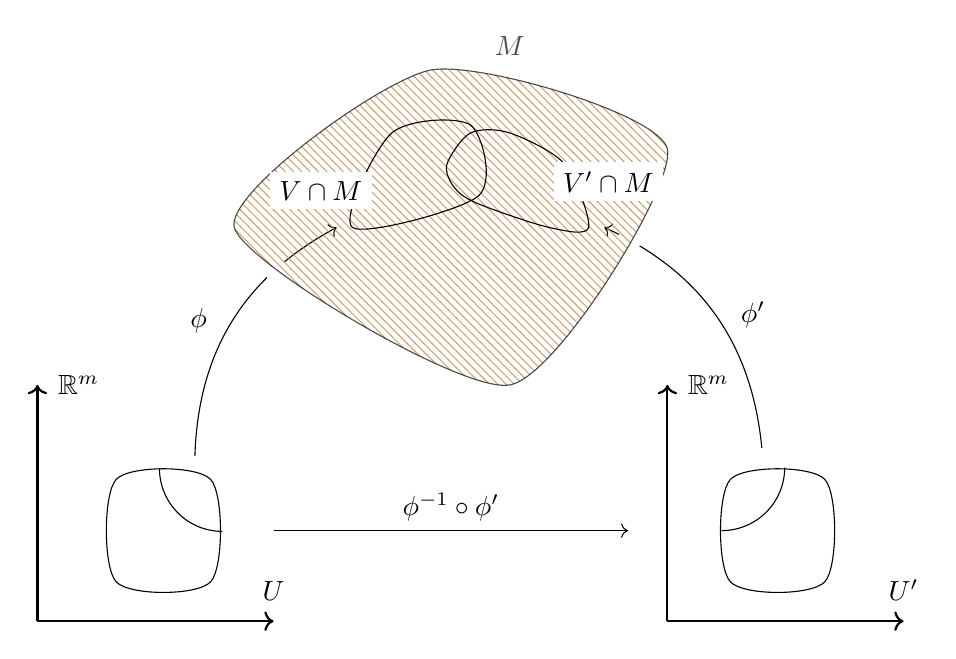
\begin{tikzpicture}

    % Functions i
    \path[->] (-1, -2.9) edge [bend left] node[left, xshift=-2mm] {$\phi$} (0.8, 0);
    \draw[white,fill=white] (0.06,-0.57) circle (.15cm);


    % Functions j
    \path[->] (6.2, -2.8) edge [bend right] node[right, xshift=2mm] {$\phi'$} (4.2, 0);
    \draw[white, fill=white] (4.54,-0.12) circle (.15cm);

    % Manifold
    \draw[smooth cycle, tension=0.4, fill=white, pattern color=brown, pattern=north west lines, opacity=0.7] plot coordinates{(2,2) (-0.5,0) (3,-2) (5,1)} node at (3,2.3) {$M$};

    % Help lines
    %\draw[help lines] (-3,-6) grid (8,6);

    % Subsets
    \draw[smooth cycle]
        plot coordinates {(1,0) (1.5, 1.2) (2.5,1.3) (2.6, 0.4)}
        node [label={[label distance=-0.3cm, xshift=-2cm, fill=white]:$V \cap M$}] {};
    \draw[smooth cycle]
        plot coordinates {(4, 0) (3.7, 0.8) (3.0, 1.2) (2.5, 1.2) (2.2, 0.8) (2.3, 0.5) (2.6, 0.3) (3.5, 0.0)}
        node [label={[label distance=-0.8cm, xshift=.75cm, yshift=1cm, fill=white]:$V' \cap M$}] {};

    % First Axis
    \draw[thick, ->] (-3,-5) -- (0, -5) node [label=above:$U$] {};
    \draw[thick, ->] (-3,-5) -- (-3, -2) node [label=right:$\mathbb{R}^m$] {};

    % Arrow from i to j
    \draw[->] (0, -3.85) -- node[midway, above]{$\phi^{-1} \circ \phi'$} (4.5, -3.85);

    % Second Axis
    \draw[thick, ->] (5, -5) -- (8, -5) node [label=above:$U'$] {};
    \draw[thick, ->] (5, -5) -- (5, -2) node [label=right:$\mathbb{R}^m$] {};

    % Sets in R^m
    \draw[white, ] (-0.67, -3.06) -- +(180:0.8) arc (180:270:0.8);
    \fill[even odd rule, white] [smooth cycle] plot coordinates{(-2, -4.5) (-2, -3.2) (-0.8, -3.2) (-0.8, -4.5)} (-0.67, -3.06) -- +(180:0.8) arc (180:270:0.8);
    \draw[smooth cycle] plot coordinates{(-2, -4.5) (-2, -3.2) (-0.8, -3.2) (-0.8, -4.5)};
    \draw (-1.45, -3.06) arc (180:270:0.8);

    \draw[white] (5.7, -3.06) -- +(-90:0.8) arc (-90:0:0.8);
    \fill[even odd rule, white] [smooth cycle] plot coordinates{(7, -4.5) (7, -3.2) (5.8, -3.2) (5.8, -4.5)} (5.7, -3.06) -- +(-90:0.8) arc (-90:0:0.8);
    \draw[smooth cycle] plot coordinates{(7, -4.5) (7, -3.2) (5.8, -3.2) (5.8, -4.5)};
    \draw (5.69, -3.85) arc (-90:0:0.8);

\end{tikzpicture}

\begin{example}[Submanifolds of $\rfield^n$]
  Let's consider some examples.
  \begin{enumerate}
    \item An open subset of dimension $n$ in $\rfield^n$ is a submanifold (by definition (a), we just take $\phi = id$). For instance $B^n\subset \rfield^n$ is a submanifold of $\rfield^n$.
    \item $S^{n-1} = \partial B^n$ is a submanifold of $\rfield^n$. Indeed, by definition (c), it is the zero set of the function:
    $$F(\underline{x}) = (x^1)^2 + (x^2)^2 + \ldots + (x^n)^2 - 1 = \underline{x}^2 -1, \underline{x} \in \rfield^n$$
    and $F_*$ is surjective: $F_*(\underline{x}) = 2 \underline{x}$
    \item $O(n) = \{A \, | \, AA^t = E\} \subset Mat(n \times n, \rfield) \cong \rfield^{n^2}$, with $E$ identity matrix. $O(n)$ is a submanifold of dimension $\frac{n(n-1)}{2}$. Indeed, using definition (c), it is the zero set of the function:
    \begin{align*}
      F \colon Mat(n \times n, \rfield) &\rightarrow Symm(n, \rfield) \\
      A &\mapsto AA^t - E
    \end{align*}
    What is more, $F_*$ is surjective. In order to prove that, we prove that "$\restrict{F_*}{A}(X)=0, \forall\, A \Rightarrow X = 0$" (then we know that for a linear map $L$ on a vector space $V$, $\dim(V) = \dim Ker(L) + \dim Ran(L)$, so the dimension of the range of $\restrict{F_*}{A}$ must be $\dim Mat(n\times n, \rfield)$, so the map is surjective).
    In fact:
    \begin{align*}
    \restrict{F_*}{A} &= \restrict{\frac{d}{dt}}{t=0}F(A + tX) = \restrict{\frac{d}{dt}}{t=0} \left[ AA^t + tAX^t + tXA^t + t^2XX^t \right] = \\
    & = AX^t + XA^t
  \end{align*}
    And the solution of:
    $AX^t + XA^t = S \in Symm(n, \rfield)$
    is $X = \frac{SA}{2}$ because $\frac{AA^t}{2}S + S\frac{AA^t}{2} = S$.
    Then:
    $$AX^t + XA^t = 0 \Longrightarrow X=0$$
  \end{enumerate}
\end{example}

Now, we want to use diffeomorphisms like those in the corollary \ref{corsubmanifold} in order to introduce the concept of manifold.

\begin{definition}[Atlas] \label{atlasdef}
  An (n-dimensional, smooth) atlas $\mathcal{A}$ on a set $M$ is a collection of maps (called charts)
  \begin{align}
    \phi_{\alpha} \colon \rfield^n &\overset{\sim}{\rightarrow} M \\
    U_{\alpha} &\mapsto W_{\alpha} \nonumber
  \end{align}
  such that:
  \begin{itemize}
    \item $\cup_{\alpha \in I} W_{\alpha} = M$
    \item $\forall\, \alpha, \beta \in I$ with $W_{\alpha} \cap W_{\beta} \not = \emptyset$,
    $$\phi^{-1}_{\beta} \circ \phi_{\alpha} \colon \phi^{-1}_{\alpha}(W_{\alpha} \cap W_{\beta}) \rightarrow \phi_{\beta}^{-1}(W_{\alpha} \cap W_{\beta})$$
    is a diffeomorphism.
  \end{itemize}
  where $\alpha \in I, I$ index set, and the $\sim$ above the arrow means that $\phi_{\alpha}$ is bijective.
\end{definition}

\begin{definition} [Equivalence relation on atlases]
  Two atlases $\mathcal{A}$ and $\mathcal{A'}$ are equivalent $\Leftrightarrow$ $\mathcal{A} \cup \mathcal{A'}$ is an atlas ($\Leftrightarrow \phi_{\beta}^{-1} \circ \phi_{\alpha}'$ is a diffeomorphism, $\forall\, \phi_{\alpha}' \in \mathcal{A}', \phi_{\beta} \in \mathcal{A})$.
\end{definition}

\begin{definition}[\textbf{Preliminary} definition of manifold] \label{manifoldprel}
  A manifold is a set $M$ with an equivalence class of atlases.
\end{definition}

\begin{remark}
  The definition \ref{manifoldprel} above is "\textit{preliminary}" because we have not specified anything about the topology yet (we are still working on Euclidean topology). Moreover, in every equivalence class $\exists!$ maximal atlas (i.e. such that, if combined with an other atlas, it can't get any bigger). We also notice that, if the charts are smooth enough, we can pullback "everything" (e.g. all our vector fields, differential forms, etc. defined for subset of $\rfield^n$). However, in that case, everything is defined \textit{locally}. In order to patch them all together, we need some other result (like the partition of unity, coming soon).
\end{remark}

\begin{example}[Projective space]
  $\mathbb{K} \in \{\rfield, \mathbb{C}\}$ ($\mathbb{K}$ is some field).
  $$\mathbb{K}P^n \equiv \faktor{(\mathbb{K}^{n+1} \setminus \{0\})}{\sim}$$
  where
  \begin{align*}&(x_0, \ldots, x_n) \sim (x_0', \ldots, x_n') \Longleftrightarrow \\
     \exists \, \lambda \in \mathbb{K}\setminus \{0\} &\text{ such that } (\lambda x_0, \ldots, \lambda x_n) = (x_0', \ldots, x_n')
  \end{align*}
  For instance, $\mathbb{C}P^1 = S^2$ (every point on a line passing through the origin is identified with the point on such line at distance 1 from the origin). We use the notation $[x_0, \ldots, x_n]$ for one equivalence class.
  Let's consider the atlas $\mathcal{A} = \{\phi_i \colon \mathbb{K}^n \rightarrow \mathbb{K} P^n \}$. Where
  \begin{align*}
    \phi_i \colon \mathbb{K}^n &\rightarrow \mathbb{K}P^n \\
    (x_0, \ldots, x_{i-1}, x_{i+1}, \ldots, x_n) &\mapsto [x_0, \ldots, x_{i-1}, 1, x_{i+1}, \ldots, x_n]
  \end{align*}
  And $\phi_i(\mathbb{K}^n) = \left\{[x_0, \ldots, x_n] \in \mathbb{K}P^n \, | \, \text{ i-th entry is } \not = 0 \right \}$.
  We notice that $\mathcal{A}$ is an atlas because $\phi_i$ satisfies the properties of the definition \ref{atlasdef}:
  \begin{itemize}
    \item $\phi$ is a bijection and its inverse is
    \begin{align*}
      \phi_i^{-1} \colon \phi_i(\mathbb{K}^n) & \rightarrow \mathbb{K^n} \\
      [x_0, \ldots, x_{i-1}, \underbrace{x_i}_{\not = 0}, \ldots, x_n] &\mapsto \left( \frac{x_0}{x_i}, \frac{x_1}{x_i}, \ldots, \frac{x_{i-1}}{x_i}, \frac{x_{i+1}}{x_i}, \ldots, \frac{x_n}{x_i} \right)
    \end{align*}
    \item $\phi$ is also a diffeomorphism, because $\phi_j^{-1} \circ \phi_i$, defined as
    \begin{align*}
      \phi_j^{-1} \circ \phi_i \colon \phi_i^{-1} \left(\phi_i(\mathbb{K}^n) \cap \phi_j(\mathbb{K}^n) \right) &\rightarrow \phi_j^{-1} \left(\phi_i(\mathbb{K}^n) \cap \phi_j(\mathbb{K}^n) \right) \\
      (x_1, \ldots, x_n) &\mapsto \Bigl( \frac{x_1}{x_j}, \ldots, \underbrace{\frac{1}{x_j}}_{i-th}, \ldots, \frac{x_n}{x_j} \Bigr)
    \end{align*}
    is a diffeomorphism (where $x_i \not = 0, x_j \not = 0$) because it is a differentiable map and the inverse is again differentiable.
  \end{itemize}
\end{example}

\begin{remark}[Extension of analysis to manifolds]
  The existence of an atlas allows us to define concepts from analysis to manifolds. For instance, we can define continuous and smooth functions on manifolds using the concepts of continuity and smoothness that we use in $\rfield^n$.
\end{remark}

\begin{definition}[Continuous/smooth function on a manifold]
  Let $M$ be a manifold, a function $f \colon M \rightarrow \rfield$ is a continuous [smooth] function if and only if $f \circ \phi_{\alpha} \colon U_{\alpha} \rightarrow \rfield$ is continuous [smooth] function $\forall \, \alpha$. Such a function is well-defined, since the definition is independent on the local parametrization chosen, thanks to the definition of atlas.
\end{definition}

\begin{remark}[cut-off functions]
  We can construct functions on a manifold in the following way: we consider a function defined on an open set in $M$ which is homeomorphic to an open set in $\rfield^n$. Then we extend it to zero outside such open set, but in order to have a differentiable function we smoothly bring it to zero using the so-called cut-off functions.
  For instance, a smooth function from $\rfield$ to $[0, 1] \subset \rfield$ such that:
  \begin{equation*}
    h(x) = \begin{cases*}
     1, & $x \le 1$ \\
     \text{anything}, &  $1 \le x \le 2$ \\
     0, & $x \ge 2$
  \end{cases*}
  \end{equation*}
  is a cut-off function.
  For example, given
  \begin{equation*}
    a(x) = \begin{cases*}
     0, & $x \le 0$ \\
     e^{-1/x}, & $x \ge 0$
  \end{cases*}
  \end{equation*}
  we can consider
  \begin{equation*}
    h(x) = 1 - \frac{a(x)}{a(x) + a(1-x)}
  \end{equation*}
  Then we use the function
  \begin{equation*}
    h_{\epsilon}(x) \equiv h \left (\frac{x}{\epsilon} \right) =
    \begin{cases*}
      1, & $x \le \epsilon$ \\
      0, & $x \ge 2 \epsilon$
    \end{cases*}
  \end{equation*}
  Now, for $p \in M$, let
  $$\phi \colon \rfield^n \supset U \rightarrow V \subset M$$
  such that $\phi(0) = p$ (where $0 \in U$) and $\epsilon > 0$ such that $B_{3 \epsilon} \supset U $. %subset?check

  \begin{figure}[H]
          \centering
  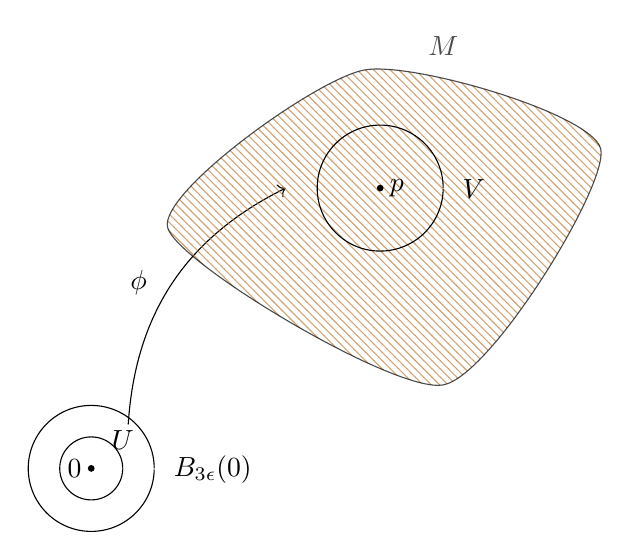
\begin{tikzpicture}
      % Functions i
      \path[->] (-1, -2.5) edge [bend left] node[left, xshift=-2mm] {$\phi$} (1, 0.5);
      \draw[white,fill=white] (0.06,-0.57) circle (.15cm);

      % Manifold
      \draw[smooth cycle, tension=0.4, fill=white, pattern color=brown, pattern=north west lines, opacity=0.7] plot coordinates{(2,2) (-0.5,0) (3,-2) (5,1)} node at (3,2.3) {$M$};

      % Help lines
      %\draw[help lines] (-3,-6) grid (8,6);

      % Subsets
      %\draw[smooth cycle]
          \draw (3, 0.5) arc (0:359:0.8) node [label=right: $V$]{};
          \filldraw[black] (2.2, 0.5) circle (1pt) node[anchor=west] {$p$};
          %\draw[white, pattern color=blue, pattern=crosshatch dots] (5.7, -3.06) -- +(-90:0.8) arc (-90:0:0.8);
          %plot coordinates {(1,0) (1.5, 1.2) (2.5,1.3) (2.6, 0.4)}
          %node [label={[label distance=-0.3cm, xshift=-2cm, fill=white]:$V \cap M$}] {};

      % Sets in R^m
      \draw (-0.67, -3.06)  arc (0:359:0.8) node [label=right: $B_{3 \epsilon}(0)$] {};
      \draw (-1.07, -3.06)  arc (0:359:0.4) node [label=above: $U$] {};
      \filldraw[black] (-1.47, -3.06) circle (1pt) node[anchor=east] {$0$};

  \end{tikzpicture}
\end{figure}
  Then $g(x) = h_{\epsilon}(|x|)$ defines a smooth function $g \colon \rfield^n \rightarrow \rfield$ with supp$(g) = \overline{\{ x \, | \, g(x) \not =  0\}} \subset U$ and $g \circ \phi^{-1} \colon V \rightarrow \rfield$ extends (by zero) to a function $f \in \mathbb{F}(M)$ with supp$f \subset V$ and $f \equiv 1$ in a neighbourhood of $p$. In particular, this shows that $\mathbb{F}(M)$ is infinite-dimensional.

  \begin{figure}
  \centering
  \begin{subfigure}{.5\textwidth}
    \centering
    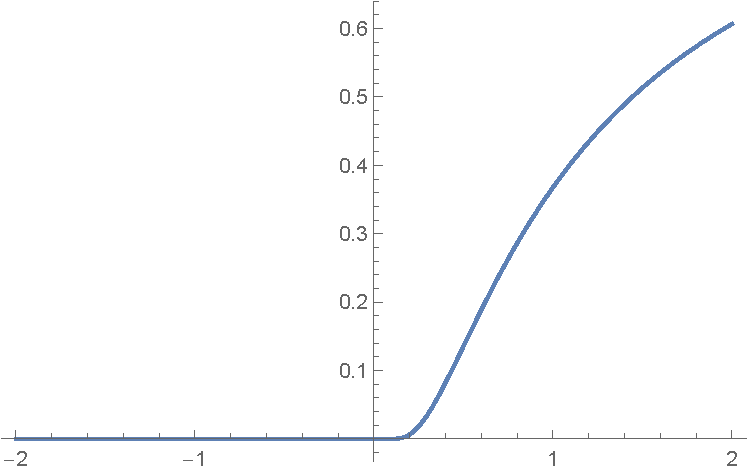
\includegraphics[width=.9\linewidth]{Images/cutoff_1.pdf}
    \caption{$a(x)$}
  \end{subfigure}%
  \begin{subfigure}{.5\textwidth}
    \centering
    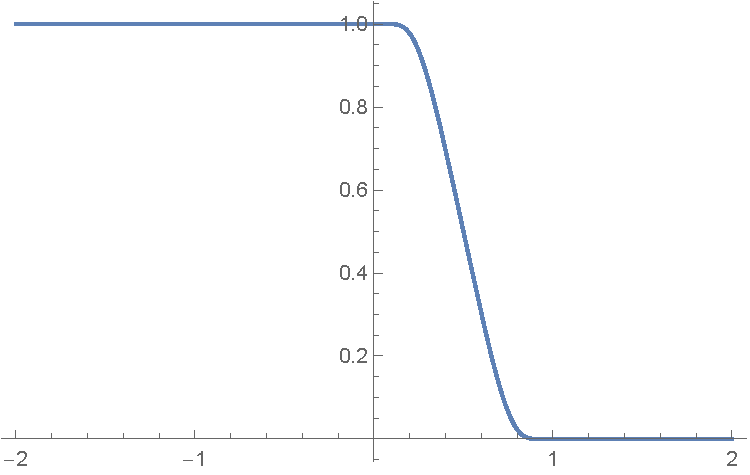
\includegraphics[width=.9\linewidth]{Images/cutoff_2}
    \caption{$h(x)$}
  \end{subfigure}
  \end{figure}
\end{remark}

\begin{definition}[Vector fields on manifolds]
  Vector fields are defined as before (we just replace $\mathbb{F}(\rfield^n)$ with $\mathbb{F}(M)$):
  $$\restrict{\Der}{p} \mathbb{F}(M) = T_p M \ni v_p \colon \mathbb{F}(M) \rightarrow \rfield$$
  And
  $$\mathfrak{X}(M) = \Der \mathbb{F}(M) = TM \ni v \colon \mathbb{F}(M) \rightarrow \mathbb{F}(M)$$
  $\rfield$-linear and satisfying Leibnitz rule.
\end{definition}

\begin{remark}[Representation of $v$ in $U_{\alpha}$]
  Everything is done in $U_{\alpha} \subset \rfield^n$ (chart). Representation of $v$ in $U_{\alpha}$:
  $$v_{(\alpha)} = v_{(\alpha)}^i \partial_{x_i}$$
  where
  $$v_{(\alpha)}^i(x) = v^i \circ \phi_{\alpha}(x)$$
\end{remark}

Notice that cut-off functions allow us to extend any smooth function on $V_{\alpha}$ (for some $\alpha \in I$) to all of $M$ through extension by zero outside $V_{\alpha}$.
Suppose we are given a function on $M$. How do we decide if it is continuous (or smooth)?
\begin{proposition}[Partition of unity]
Let $M$ be a compact manifold and let $\{V_{\alpha}\}$ be a covering of $M$. Then there exists a family of differentiable functions $\varphi_1, \ldots, \varphi_m$ such that:
\begin{itemize}
  \item $\sum\limits_{i=1}^m \varphi_i \equiv 1$
  \item $0 \le \varphi_i \le 1$ and supp$(\varphi_i) \subset V_{\alpha}$ for some $\alpha \in I$
\end{itemize}
(without proof)
\end{proposition}

\begin{remark}
  Definition of compactness for a manifold: coming soon.
\end{remark}

\begin{definition}[Partition of unity]
  The family $\{\varphi_i\}$ defined above is said to be a partition of unity subordinate to the covering $\{V_{\alpha}\}$.
\end{definition}

Now, if $f \colon M \rightarrow \rfield$, we can consider $f_i = \varphi_i f \colon v_{\alpha} \rightarrow \rfield$ for some $\alpha \in I$.

\begin{definition}[Differential forms on M]
  \begin{align}
    \Omega^k(M) \ni \omega \colon \mathfrak{X}(M) \times \cdots \times \mathfrak{X}(M) &\rightarrow \mathbb{F}(M) \\
    (v_1, \ldots, v_k) &\mapsto \omega(v_1, \ldots, v_k) \nonumber
  \end{align}
  linear, skew-symmetric (i.e. alternating) as already defined.
\end{definition}

\begin{remark}[Representation of $\omega$ in $U_{\alpha}$]
  Representation of $\omega$ in $U_{\alpha}$:
  $$\omega_{(\alpha)} = \sum\limits_{i_1 < \cdots < i_k} (a_{i_1 \cdots i_k})_{(\alpha)} dx^{i_1} \wedge \ldots \wedge dx^{i_k}$$
  where $\{x^i\}$ are the coordinates on $U_{\alpha}$.
  Moreover:
  $$\omega_{(\alpha)} ((v_1)_{\alpha}, \ldots, (v_k)_{\alpha}) = \pm \sum\limits_{i_1 < \cdots < i_k} (a_{i_1\cdots i_k})_{\alpha} (v^{i_1})_{\alpha} \cdots (v^{i_k})_{\alpha}$$
  where the $\pm$ sign depends on the orientation used.
\end{remark}

\begin{definition}[Curve on a manifold]
  A curve $\gamma \colon (a, b) \rightarrow M$ is continuous [differentiable] if $\phi_{\alpha}^{-1} \circ \gamma \colon (a, b) \rightarrow U_{\alpha}$ is continuous [differentiable]
\end{definition}
\newpage

\section{Integration of differential forms on a compact manifold}
$\omega \in \Omega^n(M), M \text{ compact manifold }, \dim M=n$. Pick a partition of unity subordinate to a covering $\{V_{\alpha} \}$ (i.e. pick some maps $\varphi_i, i=1, \ldots, n, 0 \le \varphi_i \le 1, \sum_{i=1}^m \varphi_i \equiv 1, \text{ supp}(\varphi_i) \subset V_{\alpha(i)}$ for some $\alpha = \alpha(i)$). Then:
\begin{align}
  \int\limits_M \omega &= \int\limits_M \sum_{i=1}^m \varphi_i \omega = \sum_i \int\limits_M (\varphi_i \omega) = \sum_i \int\limits_{V_{\alpha(i)}} (\varphi_i \omega) = \nonumber \\
  & = \sum_i \int\limits_{U_{\alpha(i)}} \phi^*_{\alpha(i)} (\varphi_i \omega)
\end{align}
where $V_{\alpha} = \phi_{\alpha}(U_{\alpha})$
Notice that the integral is well-defined if $M$ is orientable (definition of orientable manifolds in the next pages).

\begin{lemma}
  $\int\limits_{M} \omega$ is independent of the choice $(V_{\alpha}, \varphi_i)$
\end{lemma}

\begin{remark}
  What happens with boundaries? If $p \in \partial M$, there is no neighbourhood of $p$ homeomorphic to an open set $U \subset \rfield^n$.
  Let's define the following set:
  $$H^n = \{ (x^1, \ldots, x^n) \in \rfield^n \, | \, x^1 \ge 0 \}$$
  \textbf{Note} that on \cite{Lee} $H^n$ is defined as 
  $$H^n = \{ (x^1, \ldots, x^n) \in \rfield^n \, | \, x^n \ge 0 \}$$
  (everything is the same, but with $x^1$ replaced by $x^n$).
\end{remark}

\begin{definition}[subset topology in $H^n$]
  An open set in $H^n$ is the intersection between $H^n$ and an open set in $\rfield^n$.
\end{definition}

\begin{definition}[Functions on $H^n$]
  A function $f \colon V \rightarrow \rfield, V$ open, $V \subset H^n$ is differentiable if $\exists$ an open set $U, \rfield^n \supset U \supset V$ and a differentiable function
  $\bar f \colon U \rightarrow \rfield$ such that $\restrict{\bar f}{V} = \restrict{f}{V}$.
  Furthermore, $(f_*)_p = (\bar f_*)_p, p \in V$.
\end{definition}

\begin{definition}[\textbf{Preliminary} definition of diff. manifold with boundary]
  An $n$-dimensional differentiable manifold with a regular boundary is a set $M$ with an equivalence class of atlases, as usual, but with the difference that $\rfield^n$ in the definition \ref{atlasdef} is replaced by $H^n$ everywhere. The boundary is "regular" if it is described by a regular curve (no intersection, etc...)
\end{definition}

When is a point on the boundary of a manifold?
\begin{definition} [Point on the boundary] \label{pointbdr}
  A point $p \in M$ is on the boundary of $M$ if for some parametrisation $\phi \colon U \subset H^n \rightarrow M$ around $p$, we have $\phi(0, x^2, \ldots, x^n) = p$ for some $x^2, \ldots, x^n$.
\end{definition}%insert picture here

\begin{lemma}
  The definition \ref{pointbdr} does not depend on the choice of parametrisation.
\end{lemma}

\begin{definition} [Orientable manifold]
  $M$ is orientable if there exists an atlas $\mathcal{A} = \{\phi_{\alpha}, U_{\alpha}\}$ such that for each pair $\alpha, \beta$ with $\phi_{\alpha}(U_{\alpha}) \cap \phi_{\beta}(U_{\beta}) \not = \emptyset$, the differential
  $$
    (\phi_{\beta}^{-1} \circ \phi_{\alpha})_* \colon  U_{\beta} \rightarrow U_{\alpha}
  $$
  has positive determinant. Example of a non-orientable manifold: Möbius strip.
\end{definition}

\begin{proposition}
  \begin{itemize}
    \item The boundary $\partial M$ of a $n$-dimensional differentiable manifold with boundary is a $(n-1)$-dimensional differentiable manifold. %with boundary?check
    \item The orientation on $M$ induces an orientation on $\partial M$
  \end{itemize}
\end{proposition}

\begin{theorem}[Stokes theorem on manifolds]
  $M$ orientable, then:
  \begin{equation}
    \int\limits_M d \omega = \int\limits_{\partial M} i^* \omega
  \end{equation}
\end{theorem}

\newpage
\section{Abstract Manifolds and Topology}
\begin{remark}[Non-Example of a manifold]
The set $$M= (-\infty, 0) \cup (0, \infty) \cup \{a, b\}$$ (endowed with a particular topology that we will see later) is not a manifold. Here, $a, b$ are just two points (not necessary real numbers): just imagine $M$ as a subset of $\rfield^2$, consisting of a real line without the origin plus any two points in $\rfield^2$. Even if we have not defined a topology on $M$, we can feel that it doesn't look right: there are two maps $\varphi_a, \varphi_b$ identifying the subsets $U_a = M \setminus \{b\}$ and $U_b = M \setminus \{a\}$ with $\rfield$ (we are just calling the 0 element in other way). The transition function
$$\varphi_b \circ \varphi_a^{-1} \colon \varphi(U_a \cap U_b) = \rfield \setminus \{0\} \rightarrow \varphi_b(U_b \cap U_a) = \rfield \setminus \{0\}$$
is the identity, and is smooth. \textbf{But}  a smooth function on $M$ must have the same value when evaluated at $a$ and $b$, and this does not look right (why?).
\end{remark}

\begin{definition}[Topology] \label{top}
A topology on a set $M$ is a subset $\mathcal{O} \subset \mathcal{P}(M)$, where $\mathcal{P}(M)$ is the power set of $M$, such that:
\begin{enumerate}
	\item $\emptyset, M \in \mathcal{O}$
	\item $\mathcal{O}$ is closed under arbitrary unions: $U_i \in \mathcal{O}, i \in I$, then $\cup_{i \in I} U_i \in \mathcal{O}$
	\item $\mathcal{O}$ is closed under finite intersections: $U_1, \ldots, U_k \in \mathcal{O}$, then $U_1 \cap \ldots \cap U_k \in \mathcal{O}$.
\end{enumerate}
Sets in $\mathcal{O}$ are called open, $A \subset M$ is closed if $M \setminus A$ is open. A subset $V \subset M$ containing $p$ is a neighbourhood of $p$ if there is an open set $U \subset V$ containing $p$.
\end{definition}

\begin{remark}
From the definition above we can see that $M$ and $\emptyset$ are always both open and closed sets. Notice that a set in a topological space can be: \begin{itemize}
\item both open and closed
\item neither open nor closed
\item open but not closed
\item closed but not open
\end{itemize}
(more examples later).
\end{remark}

\begin{definition}[Closure, interior]
Let $V \subset M$, let $\mathcal{O}$ be an arbitrary topology. The closure $\bar V $ of $V$ is the smallest closed subset of $M$ containing $V$. The interior $\mathring V$ of $V$ is the largest open subset contained in $V$.
\end{definition} %TODO: existence

\begin{definition}[Continuous function, homeomorphism] \label{topcontinuity}
A map $f \colon X \rightarrow Y$ between topological spaces is continuous if $f^{-1}(U) \in \mathcal{O}_X$ for all $U \in \mathcal{O}_Y$ (i.e. if the pre-image of an open set through $f$ is still an open set). $f$ is a homeomorphism if it is bijective, continuous and $f^{-1}$ is continuous.
\end{definition}

\begin{remark}[Continuous maps vs. open maps]
Requiring that the pre-image of an open set is open is different from requiring that the image of an open set is open! If $f$ brings open sets to open sets, it is called open map (and it might not be continuous).
\end{remark}

\begin{example}
Given a set $M$, we can always consider two simple topologies on it:
\begin{enumerate}
	\item $\mathcal{O}_M =  \mathcal{P}(M)$ is a topology, where $\mathcal{P}(M)$ is the power set of $M$ (i.e. the family of all subsets of $M$). Everything is open in $M$, so it is easy to see that any function going from $(M, \mathcal{O}_M)$ to any space $(Y, \mathcal{O}_Y)$ must be continuous.
	\item $\mathcal{O}_M=\{\emptyset, M\}$ is a topology: the open sets are just the two ones required by the definition \ref{top}. In this case, every function going from any space $(Y, \mathcal{O}_Y)$ to $(M, \mathcal{O}_M)$ must be continuous (the pre-image of the empty set is the empty set, and the pre-image of $M$ is $Y$).
\end{enumerate}
What is more, we can consider topologies on metric spaces: if $(M, d)$ is a metric space and $B_{\varepsilon}(x)$ denotes the ball of radius $\varepsilon$ around $x$, then 
$$\mathcal{O}_d = \{U \subset M \, | \, \forall\, x \in U \, \exists\, \varepsilon > 0 \colon B_{\varepsilon}(x) \subset U \}$$
defines a topology. In particular, we say that the topology is induced by a metric if the open sets are the open balls of the metric space. If $X, Y$ are metric spaces, the definition of continuity seen in the Analysis courses is: $f \colon (X, \mathcal{O}_X) \rightarrow (Y, \mathcal{O}_Y)$ is continuous if and only if $\forall \, x \in X, \forall \, \varepsilon > 0, \exists \, \delta > 0$ such that $f\left(B_{\delta}(x)\right) \subset B_{\varepsilon}\left(f(x)\right)$. One can show that in metric spaces such a definition is equivalent to definition \ref{topcontinuity}.
\end{example}

\begin{remark}
If $\mathcal{O}_1, \mathcal{O}_2$ are topologies on $M$, then the intersection of the two topologies is again a topology. Therefore, given a family of subsets of $M$ one can ask for the smallest topology on $M$ which contains a subset.
\end{remark}

\begin{definition}[Hausdorff]
A topological space $(M, \mathcal{O})$ is Hausdorff if for all $p, q \in M$ there is a pair of open sets $p \in U_p, q \in U_q$ so that $U_p \cap U_q = \emptyset$.
\end{definition}

\begin{remark}
Points in Hausdorff spaces are closed sets. i.e. if $M$ is Hausdorff and $x \in X$, $\{x\}$ is a closed set. In order to see that, we just need to prove that $M \setminus \{x\}$ is open. Let's suppose $M \setminus \{x\} \not = \emptyset$ (otherwise we are done, since $M = \{x\}$ and $M$ is both closed and open). Then we can find another point $y \in M \setminus \{x\}$. Since $M$ is Hausdorff, we can find two open sets $U_x, U_y$ containing $x$ and $y$ respectively, such that $U_x \cap U_y = \emptyset$. The proof is over if we prove that $M \setminus \{x\} = \cup_{y \in M \setminus \{x\}} U_y$, since it implies that $M \setminus \{x\}$ is open (arbitrary union of open sets is open), and then $\{x\}$ is closed. It is true because:
\begin{itemize}
\item "$M \setminus \{x\} \subseteq  \cup_{y \in M \setminus \{x\}} U_y$": for each point $z$ in $M$ different from $x$, there exists an open set $U_z$ entirely contained in $M \setminus \{x\}$ by Hausdorff assumption. The point is contained in a set which is contained in $\cup_{y \in M \setminus \{x\}} U_y$ so, in particular, the point is in $\cup_{y \in M \setminus \{x\}} U_y$.
\item "$M \setminus \{x\} \supseteq \cup_{y \in M \setminus \{x\}} U_y$": if $z \in \cup_{y \in M \setminus \{x\}} U_y$, then $z \not = x$, otherwise there would be an intersection between an open set $U_{\bar x}$ for a fixed $\bar x$ and every open set containing $x$. This is impossible because by Hausdorff assumption there exists at least one open sets of those which does not intersect $U_{\bar x}$.
\end{itemize}

Moreover: 
\begin{itemize}
	\item $(M, \mathcal{P}(M))$ is always Hausdorff (there are "so many" open sets that you can always find two of them containing the right points and so that they do not intersect each other).
	\item If the topology is induced by a metric, then the topological space is Hausdorff (for instance, $\rfield^n$ with the topology induced by Euclidean metric is a Hausdorff topological space).
\end{itemize}
\end{remark}

\begin{definition}[Product topology]
Let $(M_i, \mathcal{O}_i), i \in I$ be topological spaces. Then the product topology on $\prod_{i \in I} M_i$ is the smallest topology such that all projections
$$
\prod_{i \in I} M_i \rightarrow M_j
$$
are continuous maps for all $j \in I$.
\end{definition}

\begin{definition}[Quotient topology]
Let $(M, \mathcal{O}_M)$ be a topological space and $\sim$ an equivalence relation on $M$. Then the quotient topology on $\faktor{M}{\sim}$ is the largest topology so that the function 
\begin{align*}
\pi \colon M &\rightarrow \faktor{M}{\sim} \\
x &\mapsto [x]
\end{align*}
is continuous. $\pi$ is also called canonical projection.
\end{definition}

\begin{example}[Cofinite topology]
Let $M$ be a set. We define the following topology: the open sets are $\emptyset$ and the sets $U \not = \emptyset, U \subset M$ such that their complement in $M$ is finite. Another way to define the same topology is using closed sets: the only closed sets in this topology are $M$ and the finite sets. This topology is called cofinite topology. 
$M$ with this topology is not Hausdorff if $M$ is an infinite set. 
Why? Because \footnote{the proof is easier to follow if you think of $M$ with cofinite topology as $\rfield$ endowed with cofinite topology}: given $x, y$ in $M, x \not = y$, if $U_a$ and $U_b$ are open sets that contain $a$ and $b$ respectively, the complements of $U_a$ and $U_b$ must be finite (so, $U_a$ and $U_b$ must be infinite, because the bigger space $M$ is infinite). 
But then $U_a \cap U_b \not = \emptyset$. Indeed, the complement of $U_a$ in $M$ is $M \setminus U_a$ and it must be finite because $U_a$ is open. 
If we assume $U_a \cap U_b = \emptyset$, then $U_b$ must be contained in the complement of $U_a$. But then $U_b$ (which is an infinite set, because it is open) would be contained in $M \setminus U_a$ (which is a finite set). Contradiction! 
\end{example}

\begin{lemma}
A subspace of a Hausdorff space is Hausdorff.
\end{lemma}

\begin{example}[Subspace topology]
Let $(M, \mathcal{O}_M)$ be a topological space and $N \subset M$ a subset. Then a natural topology for $N$ is the subspace (or subset) topology, defined in the following way. The subspace topology is the smallest topology so that the inclusion map $N \rightarrow M$ is continuous, i.e. $V \subset N$ is open if and only if there is an open set $U \subset M$ such that $U \cap N = V$. 

For instance, you may know that $[0, 1)$ is neither open nor closed in $\rfield$ with Euclidean topology (i.e. the topology induced by the standard metric). Actually, it is an open set in $([0, 2], \mathcal{O})$, where $\mathcal{O}$ is the subset topology (with respect to $(\rfield, \mathcal{O}_d)$, where $\mathcal{O}_d$ is the Euclidean topology). Indeed $$[0, 1) = (-1, 1) \cap [0, 2] $$
You should always pay attention to the topology and to where it is defined, for instance $[0, 1]$ is closed (but not open) in $(\rfield, \mathcal{O}_d)$, whereas it is both open and closed in $([0, 1], \mathcal{O})$, for any topology $\mathcal{O}$.
\end{example}

\begin{definition}[subbasis]
Let $M$ be a set and $B \subset \mathcal{P}(M)$ some collection of subsets. Let $\mathcal{O}_B$ be the smallest topology containing $B$, then we say that $B$ is a subbasis of $\mathcal{O}_B$.
\end{definition}

\begin{definition}[Basis]
Let $(M, \mathcal{O})$ be a topological space and $\mathcal{B} \subset \mathcal{O}$. Then $\mathcal{B}$ is a basis for $\mathcal{O}$ if every open set is a union of sets in $\mathcal{B}$.
\end{definition}

\begin{definition}[Second countability]
Let $(M, \mathcal{O}_M)$ be a topological space. Then $(M, \mathcal{O}_M)$ is second countable if it admits a countable basis.
\end{definition}

\begin{example}
Let $\mathcal{B} = \{B_{\varepsilon}(x) \, | \, \varepsilon \in \mathbb{Q}, x \in \mathbb{Q}^n \}$. This is a basis of the metric topology of $\rfield^n$ (and it is a countable set, because we used the density of $\mathbb{Q}$ in $\rfield$). 
\end{example}

\begin{lemma}
If $A \subset M$ and $M$ has a countable basis, then the subspace topology on $A$ has a countable basis.
\end{lemma}

\begin{definition}[Manifold]
A manifold $M$ of dimension $n$ is a topological space which is Hausdorff, second countable and admits an (equivalence class of) atlas(es) $\varphi_i \colon U_i \rightarrow V_i$, where $V_i$ is an open subset of $\rfield^n$ and $U_i \subset M$ is open so that the transition functions
$$\varphi_i \circ \varphi_j^{-1} \colon \varphi_j(U_i \cap U_j) \rightarrow \varphi_i (U_i \cap U_j)$$ are smooth (i.e. $C^{\infty}$). We are considering equivalence classes. we recall that the equivalence relation is the following one: two atlases are equivalent if their union is still a smooth atlas.
\end{definition}

%Add picture vector field pag. 207 Lee, and pag. 221. CHECK from page 14

\clearpage
\begin{thebibliography}{AA}
\addcontentsline{toc}{section}{Bibliography}
\bibitem{Lee}
{J.} M. Lee, Introduction to Smooth Manifolds, Springer
\bibitem{Notes}
Lecture notes (Differentiable Manifolds Saachs, Vogel WS 19)
\end{thebibliography}


\end{document}
